% v2-acmsmall-sample.tex, dated March 6 2012
% This is a sample file for ACM small trim journals
%
% Compilation using 'acmsmall.cls' - version 1.3 (March 2012), Aptara Inc.
% (c) 2010 Association for Computing Machinery (ACM)
%
% Questions/Suggestions/Feedback should be addressed to => "acmtexsupport@aptaracorp.com".
% Users can also go through the FAQs available on the journal's submission webpage.
%
% Steps to compile: latex, bibtex, latex latex
%
% For tracking purposes => this is v1.3 - March 2012

\documentclass[prodmode,acmtoit]{acmsmall} % Aptara syntax

% Package to generate and customize Algorithm as per ACM style

\usepackage[colorlinks,bookmarksopen,bookmarksnumbered,citecolor=blue,urlcolor=red]{hyperref}
\usepackage{array}
\usepackage{graphicx}
%\usepackage{caption}
%\usepackage{subcaption}

\usepackage{pifont, footnote}
%\usepackage{algorithm}
\usepackage{algorithmic}
\renewcommand{\algorithmicrequire}{\textbf{Input:}}
\renewcommand{\algorithmicensure}{\textbf{Output:}}

%\newcommand{\DCVP}{\textsc{Dcvp\xspace}}

\usepackage[ruled]{algorithm2e}
\renewcommand{\algorithmcfname}{ALGORITHM}
\SetAlFnt{\small}
\SetAlCapFnt{\small}
\SetAlCapNameFnt{\small}
\SetAlCapHSkip{0pt}
\IncMargin{-\parindent}

% Metadata Information
\acmVolume{v}
\acmNumber{n}
\acmArticle{A}
\acmYear{2016}
\acmMonth{10}

% Copyright
%\setcopyright{acmcopyright}
%\setcopyright{acmlicensed}
%\setcopyright{rightsretained}
%\setcopyright{usgov}
%\setcopyright{usgovmixed}
%\setcopyright{cagov}
%\setcopyright{cagovmixed}

% DOI
\doi{0000001.0000001}

%ISSN
\issn{1234-56789}

\newcommand\FIXME[1]{\textcolor{red}{FIX:}\textcolor{red}{#1}}

% Document starts
\begin{document}

% Page heads
\markboth{Z. Tang et al.}{Enhance Code Virtualization Protections Via Diversity}

% Title portion
\title{Enhance Code Virtualization Protections Via Diversity}
\author{Zhanyong Tang
\affil{Northwest University}
Kaiyuan Kuang
\affil{Northwest University}
Guanghui Li
\affil{Northwest University}
Di Ma
\affil{University of Michigan-Dearborn}
Dingyi Fang
\affil{Northwest University}
Xiaojiang Chen
\affil{Northwest University}
Zheng Wang
\affil{Lancaster University}}
% NOTE! Affiliations placed here should be for the institution where the
%       BULK of the research was done. If the author has gone to a new
%       institution, before publication, the (above) affiliation should NOT be changed.
%       The authors 'current' address may be given in the "Author's addresses:" block (below).
%       So for example, Mr. Abdelzaher, the bulk of the research was done at UIUC, and he is
%       currently affiliated with NASA.

\begin{abstract}
Code virtualization built upon virtual machine (VM) technologies are emerging
as a viable method for implementing code obfuscation to protect programs
against unauthorized analysis. State-of-the-art VM-based protection
approaches use a fixed set of virtual instructions and bytecode interpreters
across programs. This, however, opens up a security hole where an experienced
attacker can use knowledge extracted from other programs to quickly uncover
the mapping between virtual instructions and native code for applications
protected under the same scheme. In this paper, we propose a novel VM-code
obfuscation system to address this problem. The core idea of our approach is
to obfuscate the mapping between the opcodes of bytecode instructions and
their semantics. We achieve this by partitioning each protected code region
into multiple segments where the mapping of opcodes and their semantics is
randomized in different ways in different segments. In this way, each
bytecode instruction will be translated into different native code in
different sections of the obfuscated code. This significantly increases the
diversity of the program behavior. As a result, the knowledge of bytecode to
native code mappings obtained from other programs is unlikely to be useful
for a new program. We evaluate our approach on a set of real-world
applications and compare it against two state-of-the-art VM-based code
obfuscation approaches. Experimental results show that our simple approach is effective, 
which provides stronger protection at the cost of little extra overhead.
\end{abstract}



%
% The code below should be generated by the tool at
% http://dl.acm.org/ccs.cfm
% Please copy and paste the code instead of the example below.
%
\begin{CCSXML}
<ccs2012>
 <concept>
  <concept_id>10010520.10010553.10010562</concept_id>
  <concept_desc>Security and privacy~Software security engineering</concept_desc>
  <concept_significance>500</concept_significance>
 </concept>
 <concept>
  <concept_id>10010520.10010575.10010755</concept_id>
  <concept_desc>Security and privacy~Software reverse engineering</concept_desc>
  <concept_significance>300</concept_significance>
 </concept>
 %<concept>
  %<concept_id>10010520.10010553.10010554</concept_id>
  %<concept_desc>Computer systems organization~Robotics</concept_desc>
  %<concept_significance>100</concept_significance>
 %</concept>
 %<concept>
  %<concept_id>10003033.10003083.10003095</concept_id>
  %<concept_desc>Networks~Network reliability</concept_desc>
  %<concept_significance>100</concept_significance>
 %</concept>
</ccs2012>
\end{CCSXML}

\ccsdesc[500]{Security and privacy~Software security engineering}
\ccsdesc[300]{Security and privacy~Software reverse engineering}
%\ccsdesc{Security and privacy~Robotics}
%\ccsdesc[100]{Networks~Network reliability}

%
% End generated code
%

% We no longer use \terms command
%\terms{Design, Algorithms, Performance}

\keywords{Virtualized obfuscation, reverse engineering,
instruction set randomization, analysis knowledge}

%\acmformat{Gang Zhou, Yafeng Wu, Ting Yan, Tian He, Chengdu Huang, John A. Stankovic,
%and Tarek F. Abdelzaher, 2010. A multifrequency MAC specially
%designed for  wireless sensor network applications.}
% At a minimum you need to supply the author names, year and a title.
% IMPORTANT:
% Full first names whenever they are known, surname last, followed by a period.
% In the case of two authors, 'and' is placed between them.
% In the case of three or more authors, the serial comma is used, that is, all author names
% except the last one but including the penultimate author's name are followed by a comma,
% and then 'and' is placed before the final author's name.
% If only first and middle initials are known, then each initial
% is followed by a period and they are separated by a space.
% The remaining information (journal title, volume, article number, date, etc.) is 'auto-generated'.

\begin{bottomstuff}
%This work is supported by the National Science Foundation, under
%grant CNS-0435060, grant CCR-0325197 and grant EN-CS-0329609.

Correspondence author's Email addresses: Dingyi Fang,
%the School of Information Science and Technology,
%Northwest University, Xi��an, China, 710127.
Email: dyf@nwu.edu.cn.

Author's addresses: G. Li, K. Kuang, Z. Tang, D. Fang, X. Chen,
School of Information Science and Technology,
Northwest University, Xi��an, China, 710127;
D. Ma, Department of Computer and Information Science,
University of Michigan-Dearborn, MI, 48128;
Z. Wang, School of Computing and Communications, Lancaster University, UK.
\end{bottomstuff}

\maketitle


\section{Introduction}
Unauthorized code reverse engineering is a major concern for software developers. This technique is widely used by adversaries to perform various attacks, including removing copyright protection to obtain an illegal copy of the
software, taking out advertisement from the application, or injecting malicious code into the program. By making the program harder to be traced and analyzed, code obfuscation is a viable means to protect software against unauthorized code
modification~\cite{barak2001possibility,lynn2004positive,linn2003obfuscation,preda2005control,van2003revisiting,wu2010mimimorphism}.


Code virtualization based on a virtual machine (VM) is
emerging as a promising way for implementing code obfuscation~\cite{cv,vmp,Themida,fang2011multi,6ming2011software,wang2013nislvmp,wang2014tdvmp}.
The underlying principal of VM-based protection is to replace the program instructions
with bespoke virtual instructions and eventually encode into a bytecode program.
These virtual bytecodes will then be translated into native machine
code at runtime to execute on the underlying hardware
platform.
This forces the attacker to move from a familiar instruction set to an unfamiliar environment, which can significantly increase the time and effort involved in the attack.


Reverse engineering of VM-obfuscated code typically follows a number of steps. The attack first reverse-engineers the virtual interpreter to understand the semantics of individual bytecode instructions, i.e. how will a bytecode map be translated to native code. The attacker then translates the bytecode back to native machine instructions or even high-level program languages to understand the program logic~\cite{falliere2009inside,rolles2009unpacking}.
Among these steps, understanding the semantics of individual bytecode instructions is often the most-consuming process, which is involved in analysing the handler that used to interpret every bytecode instruction.

Numerous approaches have been proposed to protect VM handlers from reverse engineering.
Most of them aim to increase the diversity of program behavior by obfuscating the handler implementation~\cite{wang2014tdvmp} or iteratively transforming a single program multiple times using different interpretation techniques~\cite{fang2011multi,6ming2011software}.
However, all prior work employ a fixed strategy where each bytecode is deterministically translated to a fixed set of native code.
Such techniques are vulnerable for programs protected under the same obfuscation technique. In particular, an attacker can reuse the knowledge (termed \emph{\textbf{analysis knowledge}} in this paper) of the handler implementation obtained from one program to attack another program.

This paper resents DCVP (Code Virtualization Protection with Diversity), a enhanced VM-based code obfuscation system to address the issue of reusing analysis knowledge.
We employ a technique called Instruction Set Randomization (ISR)~\cite{kc2003countering} to randomly change the \textit{opcodes} of bytecode instructions and their semantics, so that the mapping
between bytecodes and their handlers will vary across programs. The randomization itself, however, is not sufficient for providing stronger protection, because it is easy to be bypassed due to the non-uniform distribution of bytecode instructions (e.g.
the more frequent a bytecode is used, the more likely the relation between the bytecode and its handlers can be obtained from other programs).
To overcome this issue, DCVP partitions the protected code region into several parts where the mappings of bytecode instructions and their handlers in each part are different. As a result, the same bytecode instruction in different parts of the bytecode program is likely to have different semantics.
It is to note that this paper focuses on protecting code against reusing analysis knowledge for code reverse engineering.
Like any code obfuscation technique, malware developers could also exploit our technique to protect malicious programs, but preventing this is outside the scope of this work.

%Of course, we have to admit that some malware authors also will use the above code virtualization technology to ``protect" their malicious code and program. For example, Themida~\cite{Themida} is a popular tool of choice. In the same way, the reverse engineer isn't always the bad guy. However, in this paper, we put ourselves in the perspective of code protection, and aims to provide a mechanism for code protection to protect the legitimate interests of users from malicious infringement.


The key contribution of this paper is a countermeasure to address the issue of reusing \textit{analysis knowledge} to perform code reverse engineering across programs.
We compare our approach against VMProtect~\cite{vmp} and Themida~\cite{Themida} on \texttt{md5.exe}, \texttt{gzip.exe}, \texttt{bcrypt.exe} and \texttt{mat\underline{ }mul.exe} applications.
Experimental results show that DCVP is able to provide stronger protection at the cost of little extra overhead.
%\FIXME{We need quantified results here. }
DCVP is similar to VMProtect in temporal and spatial overhead, and they are all better than Themida.
And on the basis of execution time costs caused by code virtualization, the growth of DCVP partitions' number hardly affects the time overhead.


The rest of the paper is organized as follows.
In Section~\ref{sec:background}, we illustrate the internals of VM-based obfuscation.
Section~\ref{sec:threat-model} gives our threat model, which describes the analyst's capabilities and goals,
and we illustrate the process of reverse engineering a VM-obfuscated program. We motivate our work in Section~\ref{sec:motivation}.
In Section~\ref{sec:overview},~\ref{sec:VIS-Handlers},~\ref{sec:NI-VI}
and~\ref{sec:VI-Bytecode}, we present the details of DCVP.
Section~\ref{sec:evaluation} evaluates DCVP for its effectiveness and its spatial and temporal overhead. Section~\ref{sec:related} presents the related work, and finally presents the conclusion and discusses the future work.
% Head 1

\section{Background}\label{sec:background}
\begin{figure}[!t]
\centering
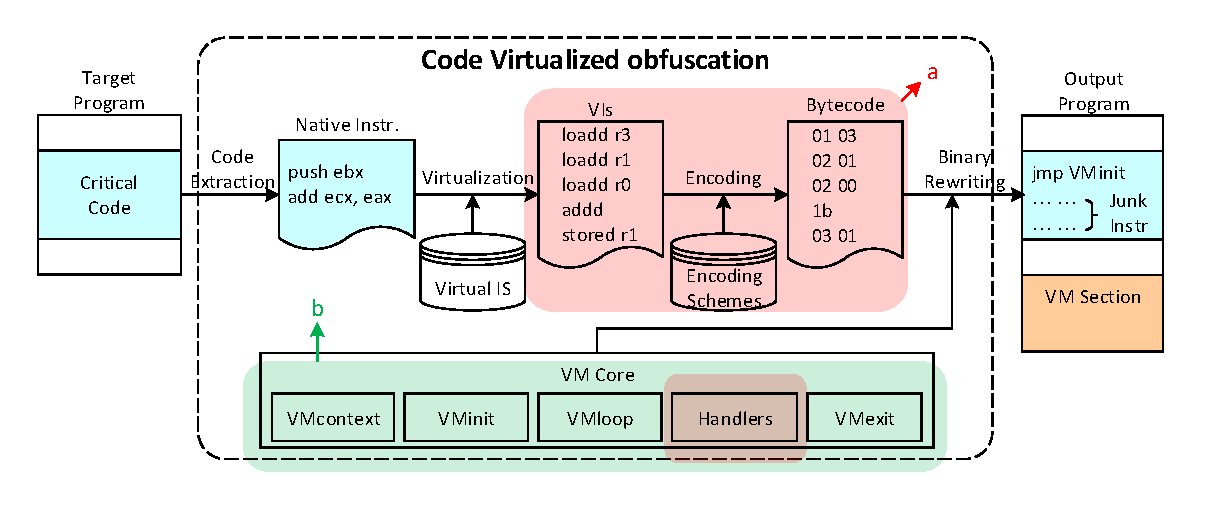
\includegraphics[width=0.9\textwidth]{fig/vmprotection.pdf}
\caption{A representative architecture for VM-based obfuscation and the execution view of a protected program. The main work of this paper is to improve the core steps of VM-based protection (areas marked as ``a" and ``b").
In the first region (a), we partition the protected code region into different segments, and obfuscate the \texttt{bytecode handlers} to generate multiple implementations for each \texttt{handler}.
In the second region, we use a number of obfuscation and anti-taint analysis technologies to protect the important components of the virtual core.}
\FIXME{Delete steps 1-4 and the left-most box. These terms are not referred anywhere in the paper.}
\label{fig:vmprotection}
\end{figure}

%Virtualization technique has been used in many fields, e.g.
%virtual memory for resource virtualization, VMware and VirtualBox for CPU virtualization,
%and Java bytecode and .Net CIL for application virtualization.
Visualization techniques is widely used to protect software programs from unauthorized analyses.
Examples of VM-based code obfuscation tools include VMProtect \cite{vmp} and Code Virtualizer \cite{cv}.
Code obfuscation often comes at a cost, with bloating code size and longer execution time.
To minimize the overhead, in practice only critical parts of the software will be obfuscated~\cite{geneiatakis2012adaptive}.
VM-based  protection works by transforming the native machine code of the protected code region into 
a set of bespoke virtual instructions (bytecode), which hopefully is unknown to the attacker. 
At runtime, the virtual instructions will be translated into native code using byte interpreters.



Figure \ref{fig:vmprotection} illustrates a classical VM-based obfuscation system. 
At the heart of this system are the virtual IS (Instruction Set) and the set of interpreters used
to translate the IS to native code.
Interpretation of virtual instructions follows the classical \textit{decode-dispatch} approach \cite{ghosh2012replacement},
using a bundle of \texttt{handlers} and a \texttt{VMloop}.
Here, the \texttt{VMloop} is the execution engine which fetches and decodes a bytecode instruction and then dispatches a \texttt{handler} to interpret instruction.
Bytecode instructions are compiled for a virtual context,  \texttt{VMcontext}, which contains hardware-independent virtual registers and flags.
At runtime, the virtual registers and flags will be mapped down to the underlying hardware. 
This work targets two key components of the VM-based obfuscation architecture, highlighted as two regions Figure \ref{fig:vmprotection} (a and b). 
Our approach divides the protected code region to different sections. It generates
multiple implementations for each bytecode handler using code obfuscation techniques. Different implementations 
of the same bytecode handler will produce an identical output for a given virtual instruction, by they follow different execution paths and exhibit 
diverse behavior during runtime. We further enhance the strength of the protection by using a number of obfuscation and anti-taint analysis technologies to protect the important components of the VMCore.



%Figure \ref{fig:vmprotection} also depicts the workflow of the obfuscation
%process. The process starts from extracting the critical code from the target
%program. This is typically done with the help of the developer who will
%mark the location and scope of the critical code to be protected during
%the development stage. The critical code section is disassembled into
%native disassembly instructions to enable later conversion from native
%instructions to virtual instructions. The rules of conversions are set ahead of time and are often fixed
%inside a VM-based obfuscation system. These rules depend on the semantics of
%the virtual IS. Subsequently, virtual
%instructions are encoded into bytecode program. Finally, the bytecode program
%and other VM components are assembled into the target program through binary
%rewriting. This paper improves the core steps of code virtualization
%protection. We modify the encoding schemes and adopt the partition bytecode
%programming, and generate multiple sets of \texttt{handlers}. So the
%bytecodes will have different semantics in different parts of bytecode
%program. We also use a variety of methods of obfuscation and anti-taint
%analysis technology to protect the critical components of virtual interpreter
%(section~\ref{sec:VI-Bytecode}).
%
%At runtime, upon executing the ``critical code", an instruction, \texttt{jmp VMinit}, transfers the control to \texttt{VMinit} (Step \ding{182}). \texttt{VMinit} saves the native context and initializes the virtual context. Next, \texttt{VMloop} starts to work. It fetches a bytecode instruction, decodes it (Step \ding{183}) and dispatches a \texttt{handler} to interpret it (Step \ding{184}). Step \ding{183} and Step \ding{184} are iterated until all the bytecode instructions are interpreted. Then, \texttt{VMloop} transfers the execution to \texttt{VMexit} (Step \ding{185}), where the native context is restored and the program jumps back to the native instruction following the critical code (Step \ding{186}) and continue to execute the rest of the program code. 

%\FIXME{I think we really need to avoid jargons here!! Everything can be explained by two short paragraphs.}

\section{Threat Model}\label{sec:threat-model}
In our threat model, we assume an attacker owns a copy of the target application and can run it in a malicious host environment \cite{collberg2002watermarking}, aka the white-box attack context \cite{chow2003white,liem2008compiler}.
In such an environment, the adversary has full privileged accesses to the system. We also assume the adversary can use static and dynamic analysis tools (such as, \texttt{IDA}~\cite{ida}, \texttt{OllyDbg}~\cite{od} and \texttt{Sysinternals Suite}~\cite{sysinternals}) to trace and analyze instructions, monitor registers and process memory, and modify instruction bytes and control flows at runtime, etc.
Prior work has demonstrated that these are reason assumptions~\cite{falliere2009inside}.
At present, there are two preliminarily used methods to attack VM-based protection systems, which are presented as follows.

The first is attack based on the virtual execution analysis proposed by Rolles et al. \cite{rolles2009unpacking}, which requires an analyst to have a certain understanding of the principle of code virtualization. By dynamically tracking the execution process of virtual interpreter to extract key bytecodes and handlers, and then through the analysis and simplify eventually recovering the original program's logic. Nicolas Falliere \cite{falliere2009inside} presented an example of the above analysis process which is used to analyze the Trojan.Clampi protected by VMProtect \cite{vmp}.
This type of attack method is closely related to the principle and structure of the code virtualization, and has the most realistic and comprehensive results.


The other one is attack based on the behavior and semantic analysis, this type of attack method can be used to attack not only code virtualization protection but also other confusion methods.
Coogan et al.~\cite{coogan2011deobfuscation} puts forward a behavior based analysis method, which aims to analyze the important behavior of code, but it does not pay attention to how to restore the original code. %This type of approach is usually used for malicious code analysis because the malicious code will interact with the system frequently in order to achieve a malicious purpose.
Yadegari et al.~\cite{Yadegari2015A} propose a method based on semantic analysis, which use taint propagation to track the flow of inputs values, and semantics-preserving code transformations to simplify the logic of the instructions.
%For the results of a run obtained, the function is equivalent to the original program, but it is only for one implementation, and does not cover all the execution branches. So the final control flow graph is only part of the original program. We need to perform analysis through multiple tracking and specify different input values each time, then comprehensive analysis to get a more complete control flow graph.
This type of method has wider applicability, but it is hard to get a comprehensive analysis results.
%So this paper mainly aims at the first kind of attack, but also will provide some measures to prevent the second kind of attack. And in our threat model, we assume that the analyst is familiar with the mechanism of code virtualized obfuscation and follows the above steps while reverse engineering a VM-obfuscated program. The ultimate goal of the analyst is to fully reverse engineer the VM-obfuscated application and automate the reverse analysis process.


\section{Motivation}
\begin{figure}[!t]
\centering
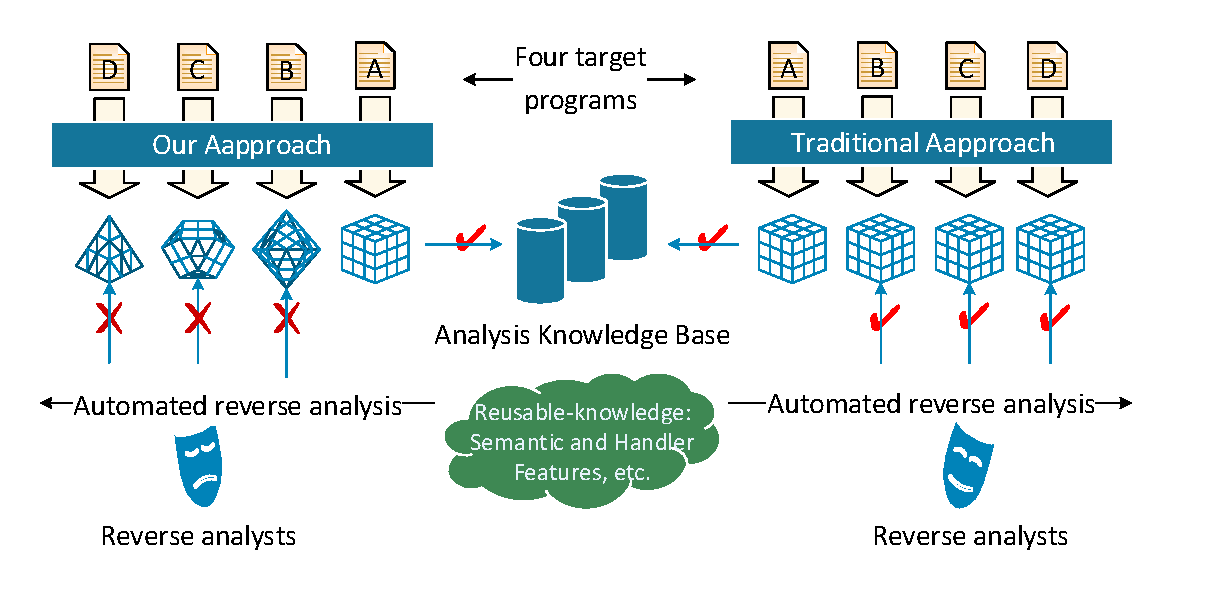
\includegraphics[width=0.75\columnwidth]{fig/figone.pdf}
\caption{The process of reusing attacking knowledge for code reverse engineering.
Here we have four different target programs, A, B, C and D.
In the right side of the scenario, all programs are obfuscated with a code obfuscation scheme that a virtual instruction will be deterministically translated to a fixed set of native code.
This allows an attacker to reuse knowledge obtained from one program to efficiently reverse engineer other programs.
In another scenario, the mapping between virtual instructions and native code is different for different programs.
In this way, the attacker is  unable to reuse the previously extracted knowledge to perform reverse analysis across programs.}
\label{fig:one}
\end{figure}

Figure~\ref{fig:one} depicts an reverse analysis scenario where an analyst can
reuse the \textit{analysis knowledge} to attack applications protected by
the same VM-based code obfuscation scheme. In this example, there are four different programs
to be protected, labelled as A, B, C and D. In the right side of the diagram,
all the four programs are protected using an identical set of virtual
instructions and bytecode handlers. Under this setting, an experienced analyst would be able to
use the knowledge of the mapping of virtual instructions and bytecode handlers obtained
from one program to reverse-engineer the other three programs. Bear in mind that,
uncovering the mapping between virtual instructions and native code is often the most
time-consuming process for attacking VM-based code obfuscation. Having able to
reuse the attacking knowledge thus can significantly reduce the cost involved in the
attack.
In another scenario, the translations between virtual instructions and native code
vary among programs. Therefore,  the
knowledge obtained from one program will be in inapplicable to others.
This forces the analyst to start from the scratch when reverse engineering a new program.
This  example shows that shuffle the relationship between the virtual instructions and bytecode handlers
can significantly increase the effort and cost involved in performing the attack.
In the remainder section, we describe how we can construct such as scheme in details.  

\section{Overview}\label{sec:overview}
DCVP consists of four components described as follows.

\paragraph{Virtual Instruction Set and Handlers}
We design a set of virtual instructions and handlers to translate the virtual instructions to native code.
In this work, we target the x86 instruction set. Our virtual instruction set is based on a stack machine architecture and is Turing-equivalent to the native machine code.
The virtual instruction set design is discussed in Section~\ref{sec:VIS-Handlers}.

\paragraph{Native code translation}
We develop a tool to automatically translate the native machine code into virtual instructions and stored as bytecode.
This is detailed in Section~~\ref{sec:NI-VI}.

\paragraph{Bytecode diversification}
The generated bytecode instructions will be diversified using a special encoding scheme.
Each protected code region is partitioned to multiple segments and the opcodes of the virtual instructions in each segment will be mapped to different native code.
This means that a mapping from opcode to native code found at one segment is likely to be inapplicable for other segments.
We also obfuscate each handler to produce a set of obfuscated handlers where handlers follow different execution paths at runtime but produce identical results for a given virtual instruction.
We also adopt anti-taint analysis to protect the core component of the VM.
This is the key component of DCVP which is presented at Section~\ref{sec:VI-Bytecode}.

\paragraph{PE Refactoring}
Finally, the generated bytecode program and other VM components will be linked together through binary rewriting.


\section{Virtual Instruction Set and Handlers}\label{sec:VIS-Handlers}
As the basis of a VM-based obfuscation system, virtual IS and the \texttt{handlers} should be the first considerations when designing such an system. The challenge lies in devising a feature-complete virtual IS that is Turing-equivalent to native IS, which means that any native instructions could be substituted with the virtual instructions. Virtual instructions ultimately will be executed by the hand-crafted \texttt{handlers}; these \texttt{handlers} are written in native instructions.

There are two main VM architectures: stack-based, and register-based. Examples of stack-based virtual machines are the Java Virtual Machine and the .Net CLR, and examples of register-based virtual machines are the Lua VM, and the Dalvik VM. In this paper, we choose stack-based architecture for the VM-based obfuscation system for the following reasons:
\begin{itemize}
  \item In a stack-based VM, operations are carried out with the help of stack, where operands and results of operations are stored. This simplifies the addressing of operands and ultimately simplifies the implementation of \texttt{handlers}.
  \item The process of converting native x86 instructions to virtual instructions is simpler.
  \item Stack-based VMs require more virtual instructions for a given computation; this makes the instructions more complex and conforms to our objective of impeding reverse analysis.
\end{itemize}

To devise a virtual IS that is Turing-equivalent to the native IS, one naive approach is devising a virtual instruction for every single native instruction. However, this results in a very large size of handlers. As the basic idea of stack-based VMs implies, a native operation are carried out or virtualized by virtual instructions in a three-phase fashion: pushing operands into the stack, executing the aimed operation, and storing the result into the virtual context. Therefore, it is sufficient for the virtual IS to include the following instructions:
\begin{itemize}
  \item \texttt{load} instructions and \texttt{store} instructions for data transfers. \texttt{load} instructions are for pushing operands into stack, and \texttt{store} instructions are for popping results out of the stack and store the results into the virtual context.
  \item Arithmetical and logical instructions. The variants of these kind of instructions are much smaller than their native ones, as the addressing mode of operands is simpler and uniform, i.e., stack-based addressing.
  \item Branch instructions for changing the control flow of bytecode program.
\end{itemize}

Other instructions that are not included in the above categories are defined as special virtual instruction - \texttt{undef}, which we will discuss later. We first discuss the different formats of these instructions and how to implement the handlers of them.

\begin{table}[]
\renewcommand{\arraystretch}{1.0}
\tbl{The Virtual Instructions and Corresponding Handlers of \texttt{load} and \texttt{store}.\label{tab:load}}{

\begin{tabular}{|l|l|}
\hline
VI              & Handler                     \\ \hline \hline
\texttt{load\underline{ }r reg}     & \texttt{movzx eax, byte [VPC]} \textit{;get vr index}     \\
                & \texttt{add VPC, 1}                  \\
                & \texttt{push dword [VMcontext+eax*4]}                  \\ \hline
\texttt{load\underline{ }r8h reg}   & \texttt{movzx eax, byte [VPC]} \emph{;get vr index}      \\
                & \texttt{add VPC, 1}                  \\
                & \texttt{movzx eax, byte [VMcontext+eax*4+1]}              \\
                & \texttt{push eax}                                      \\ \hline
\texttt{load\underline{ }m mem}     & \texttt{mov eax, dword [VPC]} \emph{;get memory addr}            \\
                & \texttt{add VPC, 4}                  \\
                & \texttt{push dword [eax]}                              \\ \hline
\texttt{load\underline{ }i8 imm8}     & \texttt{movzx eax, byte [VPC]} \emph{;get 8-bit imm value}            \\
                & \texttt{add VPC, 1}                  \\
                & \texttt{push eax}                                      \\ \hline
\texttt{load\underline{ }i16 imm16}     & \texttt{movzx eax, word [VPC]} \emph{;get 16-bit imm value}            \\
                & \texttt{add VPC, 2}                  \\
                & \texttt{push eax}                                      \\ \hline
\texttt{load\underline{ }i32 imm32}     & \texttt{mov eax, dword [VPC]} \emph{;get 32-bit imm value}            \\
                & \texttt{add VPC, 4}                  \\
                & \texttt{push eax}                                      \\ \hline
\texttt{load\underline{ }ms}        & \texttt{pop eax}                                       \\
                & \texttt{push dword [eax]}                              \\ \hline
\texttt{store\underline{ }r reg}    & \texttt{movzx eax, byte [VPC]} \emph{;get vr index}     \\
                & \texttt{add VPC, 1}                  \\
                & \texttt{pop dword [VMcontext+eax*4]}                   \\ \hline
\texttt{store\underline{ }r8h reg}  & \texttt{movzx eax, byte [VPC]} \emph{;get vr index}     \\
                & \texttt{add VPC, 1}                  \\
                & \texttt{pop edx}                                       \\
                & \texttt{mov byte [VMcontext+eax*4+1], dl}                \\ \hline
\texttt{store\underline{ }m mem}    & \texttt{mov eax, dword [VPC]} \emph{;get memory addr}               \\
                & \texttt{add VPC, 4}                  \\
                & \texttt{pop dword [eax]}                               \\ \hline
\texttt{store\underline{ }ms}       & \texttt{pop eax}                                       \\
                & \texttt{pop ebx}                                       \\
                & \texttt{mov dword [eax], ebx}                          \\ \hline
\end{tabular}
}
\begin{tabnote}
\Note{Note:}{In the table, \texttt{reg} means register, \texttt{mem} memory address, \texttt{imm} immediate value, and \texttt{vr} virtual register. \texttt{VPC} is short for Virtual Program Counter and represents the address of the next bytecode instruction to interpret.}
\end{tabnote}
\end{table}


\subsection{Load and Store Instructions}
\texttt{load} and \texttt{store} instructions are used for preparing operands and storing the results of operations. They are used in the first and third phases of virtualizing a native instruction. In our virtual IS, they are the only ones that have operands. For a \texttt{load} instruction, the operand could be a virtual register, a memory addresses, or an immediate value, and for a \texttt{store} instruction, the operand is a virtual register or a memory address. Virtual registers are stored in the virtual context, i.e., the \texttt{VMcontext}. A naive construction of \texttt{VMcontext} is simply copying the values of native registers into the \texttt{VMcontext}. But the mapping between the virtual registers and the native registers is not necessarily one-to-one. To further impede the reverse analysis, the mapping mechanism could be made purposely more complex, as NISLVMP \cite{wang2013nislvmp} does. In this section, we only consider the one-to-one mapping between the virtual registers and the native ones.



Besides the operand type, the operand size matters as well. In x86 architecture, the size of an operand could be 8-bit, 16-bit, and 32-bit. For example, given a memory address, the \texttt{load} instruction could fetch the first 8-bit, or the lower 16-bit value, or the entire 32-bit value that stored in that address. Therefore, it is better to design a virtual instruction for every distinct combination of operand type and size. However, in x86 architecture, \texttt{push} and \texttt{pop} operations do not support 8-bit operations. We decide to delay distinguishing different size operands to the second phase of virtualizing native instructions. Table \ref{tab:load} shows the virtual instructions of \texttt{load} and \texttt{store} and their corresponding \texttt{handlers}. In table \ref{tab:load}, there exists four special virtual instructions: \texttt{load\underline{ }r8h} and \texttt{store\underline{ }r8h} are used when we encounter an operation that manipulate the second least significant byte of a register, i.e., \texttt{ah}, \texttt{dh}, \texttt{ch}, \texttt{bh}. \texttt{load\underline{ }ms} and \texttt{store\underline{ }ms} have no operands and are used to process instructions with indirect memory addressing mode (memory address is stored in a register or presented as an expression). An example in table \ref{tab:native2virtual} illustrates the situation of using of \texttt{load\underline{ }ms}.

\begin{table}[!t]
\renewcommand{\arraystretch}{1.0}
\tbl{The Virtual Instructions and Handlers of \texttt{add} Virtual Instructions.\label{tab:arithmetic}}{
\begin{tabular}{|l|l|}
\hline
VI             & Handler  \\ \hline \hline
\texttt{add8}   & \texttt{pop eax}              \\
                & \texttt{add \textit{byte} [esp], al}   \\ \hline
\texttt{add16}  & \texttt{pop eax}              \\
                & \texttt{add \textit{word} [esp], ax}   \\ \hline
\texttt{add32}  & \texttt{pop eax}              \\
                & \texttt{add \textit{dword} [esp], eax} \\ \hline
\end{tabular}}
\begin{tabnote}
\Note{Note:}{Since the operations of these instructions could be 8-bit, 16-bit, or 32-bit, we design a virtual instruction for each of the operations of different operand size.}
\end{tabnote}
\end{table}


\subsection{Arithmetical and Logical Instructions}
Arithmetical and logical virtual instructions are used to execute the aimed operations and they need not to worry about operands, since their operands have been pushed into the stack by \texttt{load} instructions. However, as we said before, these instructions must consider the size of the operands. These instructions are in similar forms and we take \texttt{add} operation as an example to illustrate. Table~\ref{tab:arithmetic} lists the virtual instructions and handling procedures of \texttt{add} operation. Since the operations of these instructions could be 8-bit, 16-bit, or 32-bit, we design a virtual instruction for each of the operations of different operand size.




\subsection{Branch Instructions}
In native IS, the commonly used branch instructions include \texttt{jmp}, \texttt{jcc} (conditional jump), \texttt{call}, and \texttt{retn}. It is a big challenge to virtualize these instructions, since they have many different variants and each of these variants needs a virtual instruction. Considering the destination of a jump (branch) instruction, if its destination also resides in the critical code, we call it an \emph{inner jump}; otherwise, we call it an \emph{outer jump}. Figure \ref{fig:jump} illustrates these two kinds of branch instructions. In DCVP, we ignore the situation where the destination of a branch instruction outside the critical code resides in the critical code, the start instruction of the critical code excluded. This situation will not occur if the critical code to be protected is well-structured.

\begin{figure}[!ht]
\centering
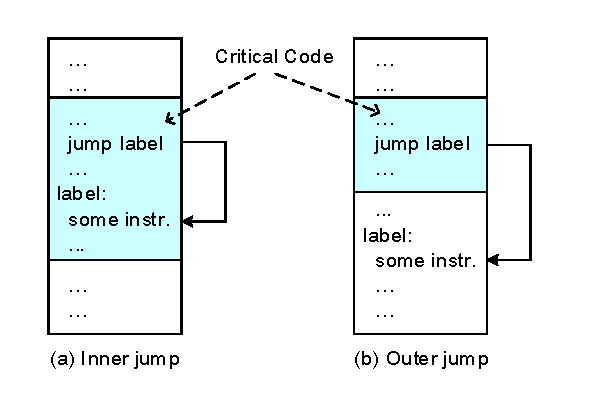
\includegraphics[width=0.45\columnwidth]{fig/jump.pdf}
\caption{The destination of a branch instruction could be in the critical code or outside the critical code. Branch instructions include \texttt{jmp}, \texttt{jcc}, \texttt{call}, and \texttt{retn}.}
\label{fig:jump}
\end{figure}

Besides the location of the destination instruction, we should also consider if the destination of a branch instruction can be determined statically. From this point of view, the branch instructions can be divided into two categories: one is \emph{direct branches}, whose destinations are calculated in a PC (Program Counter)-relative mode and can be calculated statically. The other is \emph{indirect branches}, whose destinations are stored in registers or memories. Their destinations are undefined statically and are determined at runtime. Table \ref{tab:controltransfers} classifies different forms of \texttt{jmp/jcc/call/retn} instructions considering the above two categories.

\begin{table}[h]
\renewcommand{\arraystretch}{1.0}
\tbl{Examples of Direct and Indirect Branches.\label{tab:controltransfers}}{
\begin{tabular}{|l|l|}
\hline
Direct Branches   & \texttt{jmp rel8/16/32}   \\
                           & \texttt{jcc rel8/16/32}   \\
                           & \texttt{call rel16/32}    \\ \hline
Indirect Branches & \texttt{jmp reg32/mem32}  \\
                           & \texttt{call reg32/mem32} \\
                           & \texttt{retn}             \\ \hline
\end{tabular}}
\begin{tabnote}
\Note{Note:}{In this table, \texttt{rel} means a PC-relative address. The numbers (8, 16, and 32) are the size (in bit) of the operands.}
\end{tabnote}
\end{table}


\textbf{Direct Branches}. Since \texttt{jmp} instructions are the basis of the other branch instructions, we elaborate on the introduction of the virtual instructions and handlers of \texttt{jmp} instructions. As we have illustrated, the destination of a direct \texttt{jmp} instruction can be calculated statically. If the destination instruction of the \texttt{jmp} instruction resides in the critical code, the \texttt{jmp} is a \textit{direct inner} \texttt{jmp}; otherwise a \textit{direct outer} \texttt{jmp}. We designate virtual instructions for both of them, \texttt{jmp\underline{ }di} for the former, and \texttt{jmp\underline{ }do} for the latter. For \textit{direct inner} \texttt{jmp}, it is able to obtain the corresponding bytecode instruction address of its native destination instruction during protection. Therefore, we set that bytecode instruction address as the operand of \texttt{jmp\underline{ }di}, which is pushed into stack by \texttt{load\underline{ }i}. The handler of \texttt{jmp\underline{ }di} fetches the address from stack and assigns it to VPC (Virtual Program Counter). For \textit{direct outer} \texttt{jmp}, we just need to jump to that destination instruction. Prior to that, we should restore the native context. Therefore, the operand of \texttt{jmp\underline{ }do} is the address of the native destination instruction. Table \ref{tab:jmp} presents the above two virtual instructions of \textit{direct} \texttt{jmp} and their handlers.

\begin{table}[!ht]
\renewcommand{\arraystretch}{1.0}
\tbl{The Virtual Instructions and Handlers of \texttt{jmp} Instructions.\label{tab:jmp}}{ %\texttt{jmp\underline{ }di} is for \textit{direct inner} \texttt{jmp} and \texttt{jmp\underline{ }do} for \textit{direct outer} \texttt{jmp}.}
\begin{tabular}{|c|l|}
\hline
VI                           & Handler      \\ \hline \hline %\raisebox{1.0ex}[0pt]{Handler}\\ \hline \hline
\texttt{jmp\underline{ }di}  & \emph{;operand: addr of the dest. bytecode instr.}        \\
                             & \texttt{pop eax} \emph{;get operand}                \\
                             & \texttt{mov VPC, eax}                                                \\ \hline
\texttt{jmp\underline{ }do}  & \emph{;operand: addr of the dest. native instr.}          \\
                             & \texttt{pop [mem]} \emph{;get operand}               \\
                             & \texttt{...} \emph{;restore native context}                         \\
                             & \texttt{jmp dword [mem]}                                             \\ \hline
\end{tabular}}
\begin{tabnote}
\Note{Note:}{\texttt{jmp\underline{ }di} is for \textit{direct inner} \texttt{jmp} and \texttt{jmp\underline{ }do} for \textit{direct outer} \texttt{jmp}.}
\end{tabnote}
\end{table}

\texttt{jcc} and \textit{direct} \texttt{call} instructions are similar to \textit{direct} \texttt{jmp}. \texttt{jcc} has many different kinds of instructions for different conditions, and each needs a specific virtual instruction. In the \texttt{handlers}, some extra instructions are needed to check the state of the conditions and decide to jump or not. \texttt{call} instructions can be considered as a \texttt{push} instruction followed by a \texttt{jmp} instruction. The \texttt{push} instruction pushes the return address into the stack and the \texttt{jmp} instruction jumps to the address of the subroutine.


\textbf{Indirect Branches}. Since it is difficult to obtain the address of an indirect branch, we cannot decide whether the branch is an inner one or an outer one. One solution is to delay the decision until runtime. In such case, however, the implementation of the handler is complex. Hence, for these instructions, instead of using a similar idea as that for \textit{direct branches}, we use a special virtual instruction \texttt{undef}, which will be introduced later.

\subsection{Other Instructions}
The above three categories cover the commonly used instructions. Although the other native instructions are rarely used, such as \texttt{bts}, \texttt{enter}, \texttt{int n}, and \texttt{out}, our native IS should consider them too. For these instructions, we define a special virtual instruction - \texttt{undef}. At runtime, when encountering such an instruction, it first restores the native context and exits the VM. Then, it executes that native instruction in native context and finally re-enters the VM and continues to execute the left bytecode instructions. The \textit{indirect branches} are also processed in this way.

\begin{table}[!t]
\renewcommand{\arraystretch}{1.0}
\tbl{Examples of Native Instructions and Their Corresponding Virtual Instructions.\label{tab:native2virtual}}{
\begin{tabular}{|l|l|}
\hline
Native Instr. & VI                          \\ \hline \hline
\texttt{mov eax, ebx}            & \texttt{load\underline{ }r 3}         \\
                                 & \texttt{store\underline{ }r 0}        \\ \hline
\texttt{mov eax, dword [esi+4]}  & \texttt{load\underline{ }r 6}         \\
                                 & \texttt{load\underline{ }i32 4}        \\
                                 & \texttt{add32}             \\
                                 & \texttt{load\underline{ }ms}           \\
                                 & \texttt{store\underline{ }r 0}        \\  \hline
\texttt{add eax, edx}            & \texttt{load\underline{ }r 0}         \\
                                 & \texttt{load\underline{ }r 2}         \\
                                 & \texttt{add32}             \\
                                 & \texttt{store\underline{ }r 0}        \\ \hline
\texttt{jmp 4020a8h}             & \texttt{load\underline{ }i32 42a583h}   \\
(direct inner jump)              & \texttt{jmp\underline{ }di}           \\ \hline
\end{tabular}}
\begin{tabnote}
\Note{Note:}{\texttt{42a583h} is the bytecode instruction address that corresponds to the native instruction at \texttt{4020a8h}.}
\end{tabnote}
\end{table}






\section{Native Instructions to Virtual Instructions}\label{sec:NI-VI}
At obfuscation time, we first convert native instructions into virtual instructions. This process follows a three-phase fashion: first, loading the operands into stack with \texttt{load} virtual instructions; then, executing the aimed operation; and finally, storing the result into virtual context or a certain memory address with \texttt{store} virtual instructions. Table \ref{tab:native2virtual} gives some examples of native instructions and their corresponding virtual instructions.

Data transfer instructions are mainly mapped into \texttt{load} and \texttt{store} instructions. Typical examples of these instructions are \texttt{mov}, \texttt{push}, and \texttt{pop}. Arithmetical and logical instructions strictly follow the three-phase processing. Branch instructions are mapped into a \texttt{load} instruction followed by a branch virtual instruction. Native instructions with complex addressing modes are processed iteratively with the above virtual instructions, for example, the \texttt{"mov eax, dword[esi+4]"} instruction in Table \ref{tab:native2virtual}.


\section{Virtual instructions to Bytecodes}\label{sec:VI-Bytecode}
Virtual instructions will be encoded into bytecodes in the end. It is similar to that an assembler assembles assembly instructions into machine code and only can be interpreted by virtual interpreter of VM-based protection system. We adopt an encoding scheme less compacted than the x86 instruction architecture which uses separate bytes for the \textit{opcode} and \textit{operand} of a virtual instruction. In practice, we assign each virtual instruction a distinct ID as its \textit{opcode}. The ID is used by \texttt{VMloop} as an index to find the address of the \texttt{handler} of the virtual instruction in the address table recording the addresses of each \texttt{handler}. Since the number of virtual instructions is less than 256, thus one byte is sufficient to encode their IDs. As for the \textit{operands}, since they could be of different size\footnote{The \textit{operand} of a virtual instruction could be an index for virtual register, an immediate value, or a memory address. They could be of different size: a virtual register index being 8 bits, an immediate value being 8/16/32 bits, and a memory address being 32 bits.}, we use one, two, or four bytes to encode them correspondingly. Figure \ref{fig:encoding} shows some examples of virtual instructions and their bytecode. The figure also demonstrates how \texttt{VMloop} fetches and interprets the bytecode instructions.

\begin{figure}[!t]
\centering
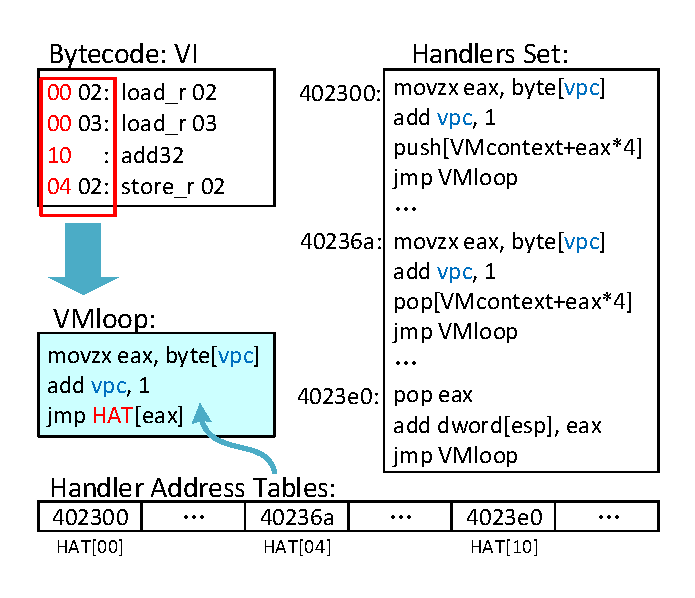
\includegraphics[width=0.4\columnwidth]{fig/encoding.pdf}
\caption{Examples of some virtual instructions and their bytecode. Each virtual instruction is encoded into a bytecode instruction, which consists of an \textit{opcode} and optionally an \textit{operand}. The bytecode instructions feed into \texttt{VMloop} and the \textit{opcode} of each bytecode instruction is used by \texttt{VMloop} as an index to find the address of the corresponding handler in the HAT (Handler Address Table).}
\label{fig:encoding}
%\vspace{-5mm}
\end{figure}

\subsection{Randomize the Semantics of Bytecode Instructions}\label{sec:random}
From the above demonstration, if an analyst gets known the semantics of a bytecode instruction, the next time she encounters it, she does not bother to analyze its \texttt{handler} once again to figure out what it does\footnote{Since \texttt{handlers} could be mutated to hinder analysis, it saves an analyst a lot of time end effort without bothering to analyze them once again.}. For example, in Figure \ref{fig:encoding}, the bytecode instruction \texttt{"10"} means an addition operation through analyzing \texttt{Handler\underline{ }4023e0}. The next time we encounter a bytecode instruction of \texttt{"10"}, we could say that it does an addition operation immediately.

To mitigate the effect of reuse of previously obtained \textit{analysis knowledge}, we randomize the semantics of virtual instructions. According to the encoding scheme we adopt, it is easy to achieve this goal. The idea is to change the relationship between the IDs (\textit{opcodes}) and the virtual instructions, which is similar to \cite{kc2003countering}. Every time to encode the virtual instructions, the IDs are first shuffled once. Then the shuffled IDs are used to encode the virtual instructions. The addresses of \texttt{handlers} are also filled into the handler address table accordingly.

\subsection{Partition Bytecode Program}\label{sec:partition-random}
With the randomization of the semantics of bytecode instructions, an analyst can not directly reuse her \textit{analysis knowlege} to work out what a bytecode instruction actually does. However, the effect of the randomization could be easily bypassed. As shown in table \ref{tab:native2virtual}, the frequencies of virtual instructions are not uniform, where \texttt{load\underline{ }r} and \texttt{store\underline{ }r} are two of the most frequently used virtual instructions. Thus, an analyst could infer the semantics of bytecode instructions based on the non-uniform frequencies of \textit{opcodes}.


\subsubsection{Bytecode Program Partition Design}
To frustrate the inferences based on the frequencies of \textit{opcodes}, we partition all the generated virtual instructions into several parts, each part been encoded differently. Specifically, during obfuscation, instead of encoding the generated virtual instructions all at a time, we encode those resulted parts separately. And prior to each encoding process, we first randomly shuffle the IDs of virtual instructions and then use the results for encoding. The effect of the shuffles is that an identical \textit{opcode} in different parts of the bytecode program probably reveals different semantics, thus the frequencies of \textit{opcodes} are obscured . Figure \ref{fig:partition} shows an example of partitioning the virtual instructions into two parts. The opcode of a virtual instruction is probably encoded differently in different parts. For example, \texttt{load\underline{ }r} is encoded into \texttt{"00"} in the first part, while \texttt{"7a"} in the other.

\begin{figure}[!t]
\centering
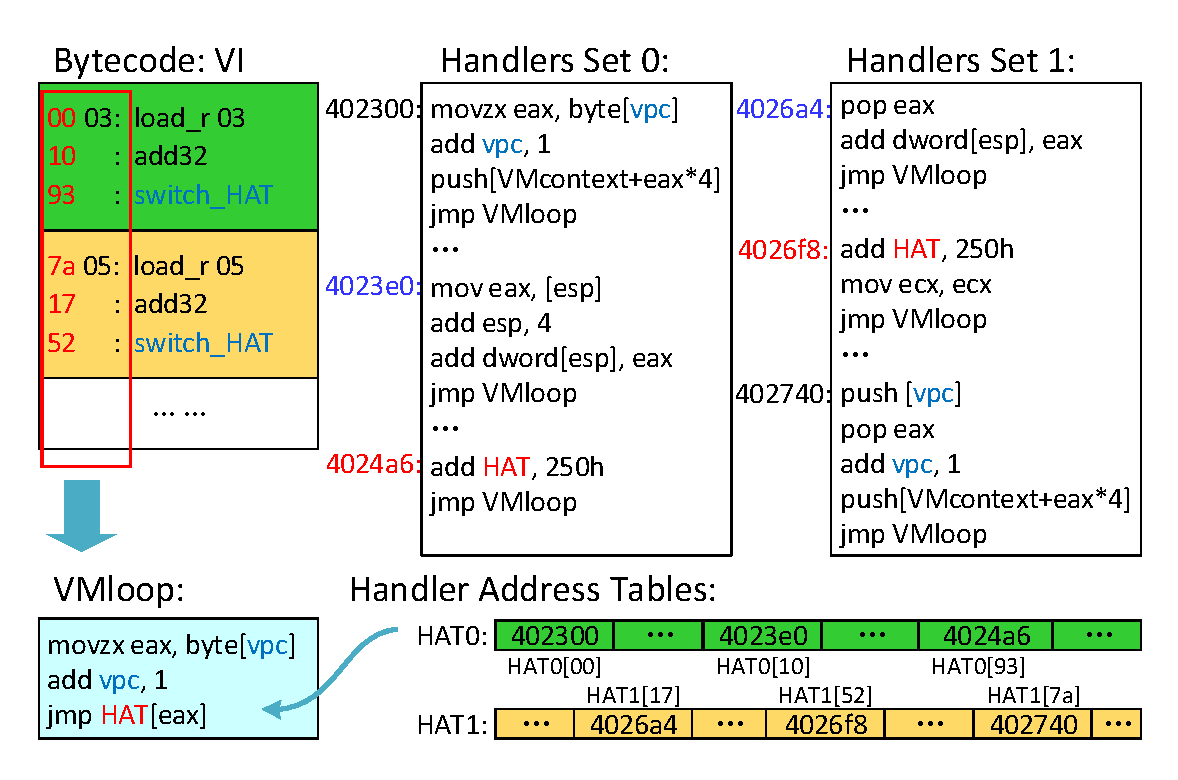
\includegraphics[width=0.55\columnwidth]{fig/partition.pdf}
\caption{Example of partitioning virtual instructions into several parts (two parts in this figure). Virtual instructions in different partitions are encoded differently and interpreted using different \texttt{handlers} set. The number of HAT increases accordingly. To switch the currently used (by \texttt{VMloop}) HAT to the next one, we add a new virtual instruction \texttt{switch\underline{ }HAT}. The \textit{operand} of \texttt{switch\underline{ }HAT} is the size of a HAT.}
\label{fig:partition}
%\vspace{-5mm}
\end{figure}

\begin{algorithm}
\caption{Partition Bytecode Program}
\begin{algorithmic}[1]
\REQUIRE VIs of critical code segment, partition number \emph{N}.
\ENSURE Bytecode program with \emph{N} partition.
\STATE Apply memory space M;
\STATE VIs randomly divided into \emph{N} partitions;
\STATE Generate \emph{N} sets of \texttt{handlers} by using algorithm~\ref{Alg:obfuscation};
\WHILE {$N \neq 0$}
\STATE Take a partition;
\STATE Randomly select a set of \texttt{handlers} and shuffle the IDs of virtual instructions;
\STATE Build a corresponding HAT;
\STATE Use the shuffle results to encode bytecode program P;
\STATE Store the P to M;
%\STATE \emph{N} decrement operation
\STATE $N--$ ;
\ENDWHILE
\end{algorithmic}
\label{Alg:partition}
\end{algorithm}

Algorithm~\ref{Alg:partition} demonstrated the implementation of the partition encoding. Partition the bytecode program, we will randomly divide virtual instructions into \emph{N} partitions and obfuscate the original HAS (Handler Set) for N times to get N sets of \texttt{handlers}, and the detailed HAS obfusction approach are demonstrated in section~\ref{sec:multi-handler}. For each partition, we will randomly select one set of \texttt{handlers} and shuffle the IDs of virtual IS, and then use the results to encode the VIs into a specific bytecode program. In the end, a complete bytecode program is generated, which has multiple partitions and the same bytecode has different semantics in different partitions. These specific bytecodes only can be can be interpreted by system's virtual interpreter.
%which contains \texttt{VMloop}, HAT and HAS.




As the \textit{opcodes} of bytecode instructions are used by \texttt{VMloop} as the indexes for the addresses of their corresponding \texttt{handlers}, and different partitions are encoded differently, each partition needs their own HAT. At the end of a partition, the HAT used by \texttt{VMloop} should be switched to the HAT of the next partition. This is done by a new virtual instruction - \texttt{switch\underline{ }HAT}. Since \texttt{switch\underline{ }HAT} is always added to the end of a partition and the orders of HATs are in accordance with that of the partitions, \texttt{switch\underline{ }HAT} needs to add the size of a HAT to the HAT pointer used by \texttt{VMloop} (as \texttt{Handler\underline{ }4024a6} does in figure \ref{fig:partition}). In our prototype, the number of \texttt{Handlers} is \texttt{148} and the address of a \texttt{Handler} is \texttt{4} bytes, thus the size of a HAT is \texttt{592} (\texttt{250h in hexadecimal}) bytes.

\begin{figure}[!t]
\centering
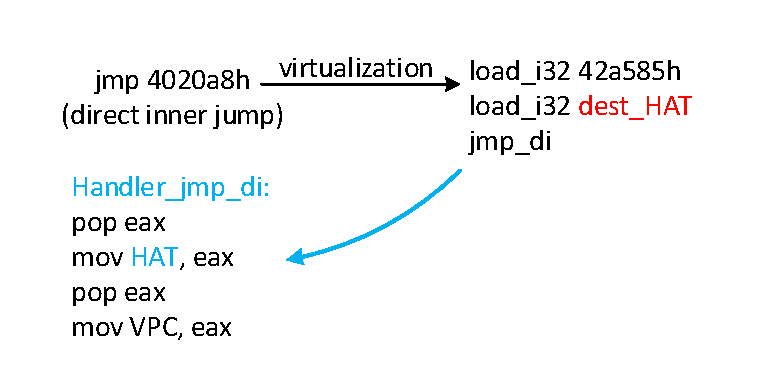
\includegraphics[width=0.5\columnwidth]{fig/directjmp.pdf}
\caption{The virtualization of a \textit{direct inner} transfer instruction with HAT switching. The address of the destination HAT is pushed into stack by \texttt{load\underline{ }i}, and is assigned to the HAT pointer used by \texttt{VMloop} at runtime.}
\label{fig:directjmp}
%\vspace{-5mm}
\end{figure}


The switchings of HATs is not limited to the end of partitions. A branch instruction also causes the switching when its destination resides in a different partition. Branch instructions change the control flow of a program through changing the VPC. When encounter such an instruction, we cannot simply append a \texttt{switch\underline{ }HAT} to it, since the \texttt{switch\underline{ }HAT} may not get interpreted by \texttt{VMloop} if the VPC is changed to a location in another partition. Hence, we put the code for switching inside the \texttt{Handlers} of the branch instructions. Here, the branch instructions indicate the \textit{direct inner} ones, as \textit{direct outer} branches and \textit{indirect} branches all leave the virtual context and need not to worry about the switching of HATs. During protection, for each \textit{direct inner} branch instruction, we first calculate its destination, and then figure out which partition the destination resides. The address of the HAT of that partition is pushed into stack by \texttt{load\underline{ }i} and will be used by the \texttt{Handler} of the branch instruction to set the value of the HAT pointer used by \texttt{VMloop}. Figure \ref{fig:directjmp} shows the virtualization of a \textit{direct inner} branch instruction, compared to that in table \ref{tab:jmp}.


\subsubsection{Security Analysis of Partition Design}
Assume there is an attacker now, which uses the attack method based on virtual execution that introduced in section~\ref{sec:threat-model} to reverse the partition bytecode program. First, the attacker needs to perform dynamic debugging the target program, and then spend some time to locate the address of \texttt{VMloop} from the obfuscated virtual interpreter. Next he needs to collect the bytecode program by analyzing the parameters of \texttt{VMloop}.

To restore the logical function of the original code, the attacker needs to analyze the semantics of these extracted bytecodes. But for the target program, which generated by using a special encoding schemes and its bytecode program is divided into multiple partitions. So the attacker must first obtain the partition informations of critical code to further reverse analysis, but it is difficult for him. After the NIs is converted to a VIs, there is a HAT switching operation by using VI - \texttt{switch\underline{ }HAT} at the end of each partition. However, virtual instruction is just an intermediate language in the process of protection, and it does not appear in the final program. All of the instructions will eventually be in the form of bytecodes, and the bytecode semantics of each partition is randomly changed (such as bytecode ``93" and ``52" in figure~\ref{fig:partition}). So the attacker cannot use this feature to delineate the partition. He can only spend a lot of time through continuous tracking and debugging to predict the partition of the transformation.

Assume that the attacker gets the partition information after a lot of analysis. Next the attacker need to analyze the bytecode of each partition and extract the semantic information implied by the \texttt{handlers}. Because the bytecode of each partition has a different semantics, and their mapping \texttt{handlers} are also with different forms. Therefore, the attacker cannot reuse the previous \textit{analysis knowledge} to attack the next partition, and for different target program that protected by DCVP is more like this. Unique partition configuration and different \texttt{handler} sets, so that the attacker cannot achieve the batch automatic attack by building attack knowledge base. The attacker has to spend a lot of time to analyze every detail for each program.





\subsection{Obfuscate the Handler Sets}\label{sec:multi-handler}
To further impede automated reverse analysis, we can obfuscate the \texttt{handlers}, and use different obfuscation strategies for \texttt{handlers} in different partitions. As a result, a \texttt{handler} in different partitions will looks different. An analyst cannot immediately recognize them as the the same one and needs to analyze each of them, which increases the workload of the analyst. At the same time also can prevent the attacker use attack knowledge base to match these \texttt{handlers} to achieve automated reverse analysis.

\begin{algorithm}
\caption{Virtual Interpreter Obfuscation}
\begin{algorithmic}[1]
\REQUIRE The original HAS, partition number \emph{N}.
\ENSURE \emph{N} equivalent HASs with different forms.
\WHILE {$N \neq 0$}
\STATE Apply memory space M1;
\STATE Take the first \texttt{handler} from HAS;
\WHILE {There are still untreated \texttt{handler}}
\STATE Randomly select multiple obfuscation methods and using order of them;
\STATE Obfuscate \texttt{handler} and store the results to M1;
\STATE Take the next \texttt{handler} from HAS;
\ENDWHILE
\STATE Apply memory space M2;
\STATE Using the anti-taint analysis technique to protect the code in M1;
\STATE Store the results to M2, and release the memory space of M1;
%\STATE \emph{N} decrement operation
\STATE $N--$ ;
\ENDWHILE
\end{algorithmic}
\label{Alg:obfuscation}
\end{algorithm}

The obfuscation approach we take is shown in Algorithm~\ref{Alg:obfuscation}. The number of HAS obfuscated is determined by the number of partitions. Our system will randomly select several methods from the obfuscation method library which contains the junk instructions injection, equivalent instruction substitution~\cite{nicolaou2009applied}, code out-of-order~\cite{Birrer2007Program} and control flow flattening~\cite{Wang2001Protection}. Then the system will use the selected method in a random order to obfuscate the \texttt{handler}. Finally we have multiple equivalent but different forms of HASs. We will also adopt some anti-taint analysis techniques (some details are presented in section~\ref{sec:anti-taint}) to protect the HASs that after obfuscated. This can effectively prevent the virtual interpreter from being attacked by some de-obfuscation methods.


For example, HAS (Handler Set) as an original \texttt{handler} set that consists of \emph{m} \texttt{handler}. We use a HAT to store the address of these \texttt{handlers}, and their index corresponds to the \textit{opcode} of virtual instruction. HAS will be obfuscated for \emph{n} times with different strategies, \emph{n} is dependent on the number of partitions. Then we get multiple HASs and which are semantic equivalence but have different forms. At this time, all of the equivalent \texttt{handlers} still have the same index. This is a type of insecure and direct mapping relationship. Therefore, according to the method that partition bytecode program and randomized the semantics of bytecode instructions in the upper section~\ref{sec:partition-random}, we first randomly shuffle the IDs of virtual instructions and then use these results to generate a new HAT for each partition (as shown in figure~\ref{fig:partition}). The effect of shuffles is that an identical \textit{opcode} in different parts of the bytecode program probably reveals different semantics. The relationship of these equivalent \texttt{handlers} in different HASs should be:
\[\emph{HAS$_1$(i)$\Leftrightarrow$HAS$_2$(j)$\Leftrightarrow$ ... $\Leftrightarrow$HAS$_{n}$(k), 1$\leq$i, j, k$\leq$m}.\]
This various semantics of bytecode instructions and different forms of \texttt{handlers} can effectively prevent the attacker from using the attack knowledge base matching to realize the automated reverse analysis. The attacker has to spend a lot of time to analyze every detail.


\begin{figure}[t]
\centering
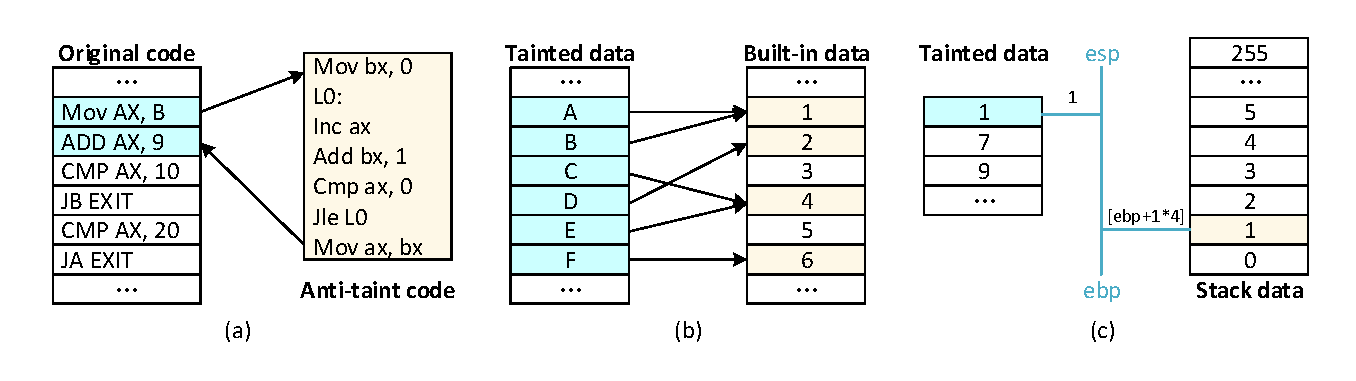
\includegraphics[width=0.9\textwidth]{fig/figanti-taint.pdf}
\caption{Examples of three anti-taint analysis techniques. Respectively as, (a) the transfer of naive model, (b) the transfer of control dependencies and (c) the indirect transfer of stack pointer.}
\label{fig:anti-taint}
\end{figure}

\subsection{Anti-Taint Analysis \label{sec:anti-taint}}
Simply obfuscating the \texttt{handlers}, however,
cannot prevent an attacker from reverse engineering completely.
There are several existing de-obfuscating techniques that
can be used to counter the traditional virtualization protection.
Such as, Coogan et al.~\cite{coogan2011deobfuscation}, who use equational reasoning
about assembly-level instruction semantics to simplify away obfuscation code from
execution traces of emulation-obfuscated programs.
Yadegari et al.~\cite{Yadegari2015A}, which use taint propagation to track
the flow of values from the program��s inputs to its outputs,
and semantics-preserving code transformations to simplify the logic of
the instructions that operate on and transform values through this flow.

However, the work of Coogan et al. is based on equational reasoning about assembly level instruction semantics,
and it is difficult to simplify the complex equation,
that making it hard to separate out the different components of nested loops or complex control flow.
%Besides, this is a kind of behavior based analysis method, which has good applicability to the analysis of malicious code, but the result of the analysis of the benign program is not good. The results can not fully reflect the function of the protected code.
The work of Yadegari et al. can be effective even when applied to previously unseen obfuscations, but code simplification should be first to identify input-to-output data flows. This rely on the taint propagation and analysis to identify the explicit flow of values from inputs to outputs, then use control dependence analysis to identify implicit flows. Therefore, these methods may be impeded by enforcing dataflow obfuscation to the handling procedures~\cite{liem2008compiler}. We adopt some anti-taint analysis techniques to protect the data flow of the \texttt{handlers} from taint analysis. Specific ways are as follows:

\paragraph{The transfer of naive model}
A simple case is given in Figure~\ref{fig:anti-taint}-(a), assuming that there is a variable \emph{B} that has been marked by taint, we need to transfer the value of \emph{B} to \texttt{AX}. If we use the \texttt{MOV} instruction, \texttt{AX} will also be tainted. The transfer of naive model is that to do subtraction operation for \emph{B}, at the same time to do addition operation for \texttt{AX}. When the value of \emph{B} is reduced to "0", the value of AX increased from "0" to \emph{B}, and \texttt{AX} will not be marked as a tainted data.

\paragraph{The transfer of control dependencies}
Control dependence analysis is an important step towards the process of taint analysis. For a set of tainted data, to carry out anti-taint analysis processing. As shown in Figure~\ref{fig:anti-taint}-(b), we can launder tainted data by assigning the data that non tainted directly to the tainted data. This process needs to match the tainted data and not tainted data, in order to ensure the correctness of the data will not be affected.

\paragraph{The indirect transfer of stack pointer}
As we can see from Figure~\ref{fig:anti-taint}-(c). The indirect transfer of stack pointer took advantage of the working principle of the stack to implement the anti-taint analysis. The principle of this method is to first put a set of non tainted data into the stack, and then through the address pointer of stack data to access the stack data, and finally use the stack data to replace the tainted data to implement the anti-taint analysis.

The above three methods can prevent the spread of tainted data by laundering tainted data
and resist the taint analysis effectively .


\section{Evaluation}\label{sec:evaluation}
In this section, we first evaluate the effectiveness of DCVP by computing the likelihood of a bytecode instruction of two partitioned segments is mapped to identical machine code. We then evaluate the overhead of DVCP in terms of the code size and runtime.


\subsection{Effectiveness Evaluation}
DCVP is effective for impeding reverse analysis by invalidating existing \textit{analysis knowledge}.
From Section~\ref{sec:background}, we learned that understanding the semantics of bytecode instructions
is essential for reverse engineering a VM-obfuscated program.
Semantics are encapsulated in \texttt{handlers}, and the work of extracting them
form \texttt{handlers} is tedious and error-prone.
Therefore, it will save analysts lots of time and energy if the semantics of bytecode instructions are accessible,

\begin{figure}[!t]
\centering
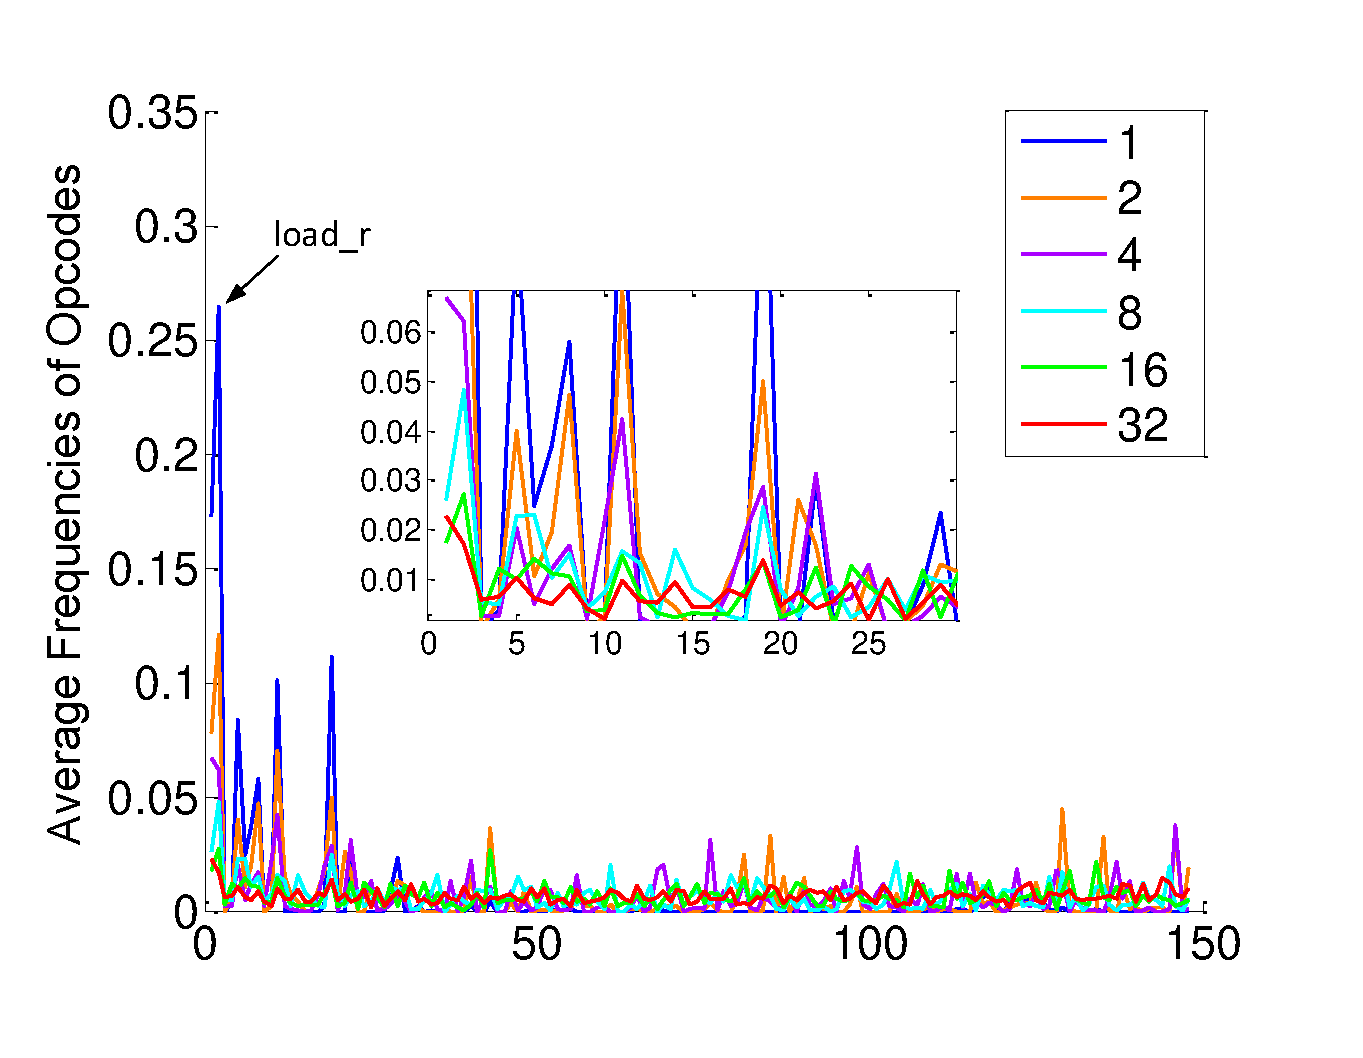
\includegraphics[width=0.5\textwidth]{fig/opfreq.pdf}
\caption{The average frequencies of \textit{opcodes}. The horizontal axis specifies the \textit{opcodes}.}
\label{fig:freq}
\end{figure}

without bothering to trace and analyze the \texttt{handlers} once again.
DCVP's aim is to frustrate this attempt and force analysts to analyze the \texttt{handlers} every time.
Through randomizing the semantics of bytecode instructions,
the same bytecode instruction probably means different obfuscated instances,
and even different in the same obfuscated program by adopting different encoding schemes
for different partitions of the bytecode program,
which can largely confuse analysts and increase their workload.


Assuming that the number of virtual instructions, or the number of \texttt{handlers} in other words, is $H$,
then the probability of a bytecode instruction in two obfuscated programs having the same semantics is $\frac{1}{H}$.
The total number of distinct shuffle of the \textit{opcodes} is $H!$. In an obfuscated program,
supposing the bytecode program is partitioned into $N$ parts,
then the probability that a bytecode instruction in different partitions having
the same semantics is $\left(\frac{1}{H}\right)^{N-1}$.
Therefore, we believe DCVP can effectively remove the \textit{analysis knowlege}
about the semantics of bytecode instructions.

We also put the four target programs (Table~\ref{tab:statistics}) together 
and count the average frequencies of \textit{opcodes}.
We take the obfuscated programs with 1, 2, 4, 8, 16, and 32 partitions for comparison.
The results are presented in figure \ref{fig:freq}.
As we can see, as the number of partitions increases,
the frequencies of \textit{opcodes} tend to be closer.
When the partition number is 1, we can easily get the instruction
that has the highest frequency is ``\texttt{load\underline{ }r}",
since it is the most commonly used instruction.

\subsection{Overhead Evaluation}
To evaluate the spatial and temporal overhead of our method, we implemented a prototype,
namely DCVP, for obfuscating x86 PE executables on the Windows platform.
In the implementation, we devised \texttt{148} virtual instructions and their corresponding \texttt{handlers}.
We conducted all the experiments on a Dell Optiplex 960h with
an Intel\textregistered Core\textsuperscript{TM} 2 Duo Processor E8400 at 3.00GHz with 4.00GB of RAM.
The operating system environment is Windows 7 Enterprise.


We use DCVP to protect four x86 PE executables,
namely \texttt{md5.exe}\footnote{MD5: Command Line Message Digest Utility. http://www.fourmilab.ch/md5/.},
\texttt{gzip.exe}\footnote{gzip. http://www.gzip.org/\#sources.},
\texttt{bcrypt.exe}\footnote{Bcrypt - Blowfish file encryption. http://sourceforge.net/projects/bcrypt/.},
\texttt{mat\underline{ }mul.exe}\footnote{Matrix multiplication. https://github.com/MartinThoma/matrix-multiplication.}.
The first three are used to process a text file (\texttt{test.txt}) of 10KB
and \texttt{mat\underline{ }mul} is used to calculate the product of two 5$\times$5 matrices.
Table \ref{tab:statistics} shows the statistics of these executables.
For each program, we choose a piece of critical code to protect, as shown in table \ref{tab:statistics}.
The programs are protected 10 times, each time with a parameter that specifies a different number (1$\sim$10) of partitions.


\begin{table}[!t]
\renewcommand{\arraystretch}{1.1}
\tbl{Statistics of the Target Programs.\label{tab:statistics}}{
\begin{tabular}{|l|l|r|l|c|r|c|c|}
\hline
Target Program  & Version & Size(KB) & Critical Code & N1 & N2 & Ratio & N3 \\ \hline\hline
md5.exe         & 2.3     &  11      & Transform()         & 1327 &  563  & 42.36\% &   85013 \\ \hline
gzip.exe        & 1.2.4   &  56      & deflate()           & 10181 & 153  & 1.50\%  &  539082 \\ \hline
bcrypt.exe      & 1.1.2   &  68      & Blowfish\underline{ }Encrypt() & 2997 & 54 & 1.80\% & 1735710 \\ \hline
mat\underline{ }mul.exe & - & 184    & ijkalgorithm()      & 49327 & 60   & 0.12\%        &   84325 \\ \hline
\end{tabular}}
\begin{tabnote}
\Note{Note:}{%The 4th column indicates the critical function we choose to protect for each program.
The 5th and 6th column gives the number of instructions in the entire program and these critical functions respectively, The 7th column gives the proportion of critical code.
We use Pin~\cite{pin} to count the number of the dynamically executed instructions in the critical functions and the results are shown in the last column. We chose only 60 instructions of \texttt{mat\underline{ }mul} is special to verify the impact of DCVP on the program overhead when protecting a small amount of code. The results are shown in figure~\ref{fig:runtime} and the impact is not obvious.}
\end{tabnote}
\end{table}



\begin{figure}[t]
\centering
\begin{minipage}[t]{0.32\linewidth}
\centering
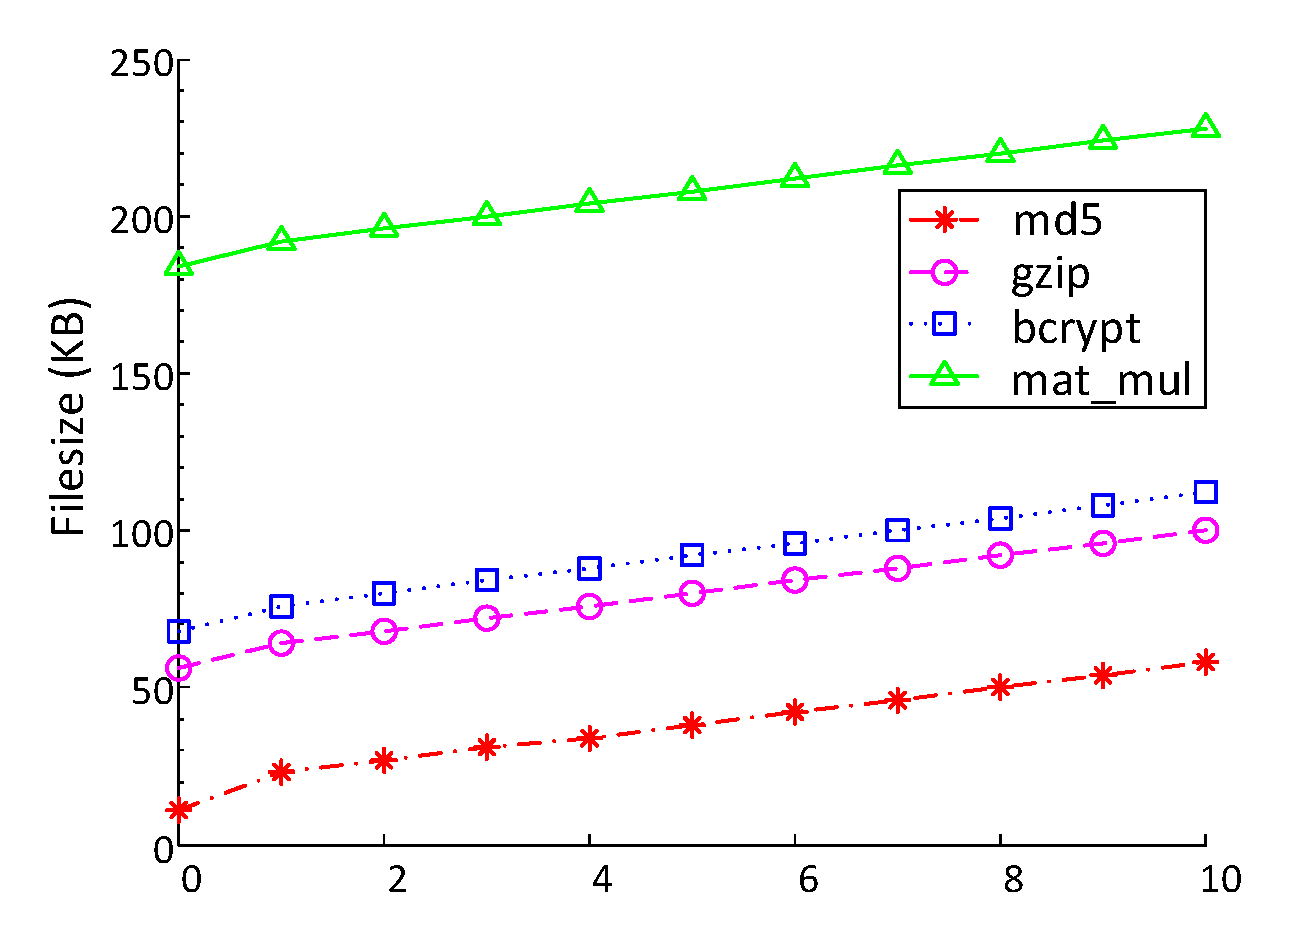
\includegraphics[width=0.9\textwidth]{fig/filesize.pdf}
\caption{The impact on code size (KB) of DCVP. The file size slightly increased with the increase of number of partitions}
\label{fig:filesize}
\end{minipage}
%\end{figure}
\hspace{0.005\textwidth}
\begin{minipage}[t]{0.32\linewidth}
%\begin{figure}[t]
\centering
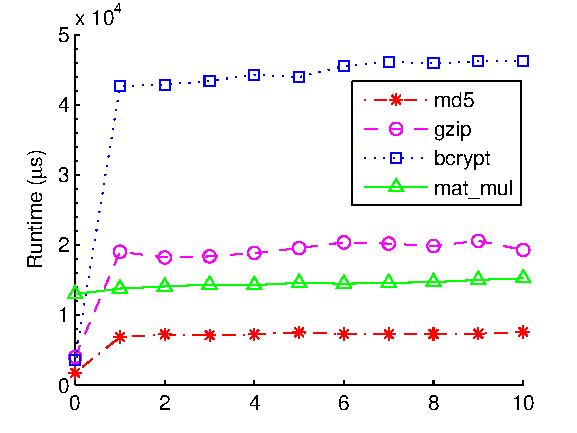
\includegraphics[width=0.9\textwidth]{fig/runtime.pdf}
\caption{The impact on runtime performance ($\mu$s) of DCVP with different partitions.}
\label{fig:runtime}
\end{minipage}
\hspace{0.005\textwidth}
\begin{minipage}[t]{0.32\linewidth}
\centering
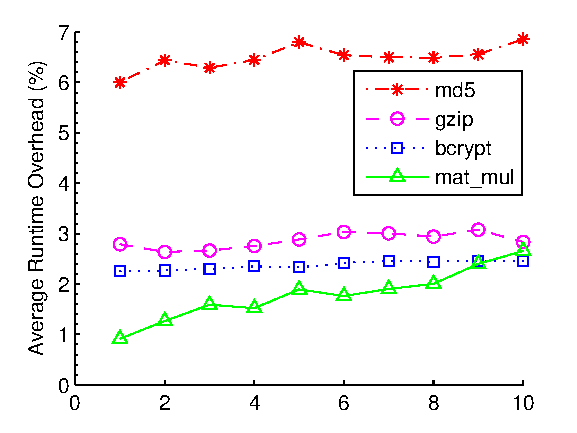
\includegraphics[width=0.9\textwidth]{fig/avg_runtime.pdf}
\caption{The average runtime overhead per dynamically executed critical instruction.}
\label{fig:avgruntime}
\end{minipage}
\end{figure}


Figure \ref{fig:filesize} shows the code size of the obfuscated programs.
The horizontal axis specifies the number of partitions in the obfuscated programs
and ``\texttt{0}" means the original program.
As the partitions increase, the increased bytes mostly come from the added HATs and HAS.
Since the size of a HAT is only 592 bytes, the sizes of the HATs increase slowly.
Besides, the sections in PE executables are aligned to a value (4096 or 512 usually)\cite{pe},
the filesize of the program is mainly affected by the number of HAS,
and it increases with the increase of partition's number regularity.


To evaluate the runtime overhead that DCVP introduces,
we run the obfuscated programs for several times and calculate the average execution time of them:
\texttt{md5}, \texttt{gzip}, and \texttt{bcrypt} are used to process a text file (\texttt{test.txt}) of 10KB; \texttt{matrix\underline{ }mul} is used to calculate the product of two 5$\times$5 matrices.
The average execution time is shown in figure \ref{fig:runtime}.
Among them, \texttt{bcrypt} has the largest increase of execution time from original
program\footnote{The execution time of the original program is specified by ``\texttt{0}" on the horizontal axis.}
to the obfuscated program with one partition.
This resulted from that the critical instructions in \texttt{bcrypt} is executed much more times
than others (as shown in the last column in table \ref{tab:statistics}).
Besides, the execution time changes little as the number of partitions increases.
From section~\ref{sec:partition-random} we can learn that if the number of partitions increases by one,
the program only needs to execute an extra \texttt{handler} to interpret the \texttt{switch\underline{ }HAT} instruction.
The introduced runtime overhead is negligible.
In some situations, the execution time of an obfuscated program with more partitions
may have a slightly lower runtime overhead.
This probably results from the locality of reference\footnote{Locality of reference. https://en.wikipedia.org/wiki/Locality\_of\_reference}. %\cite{locality}.

%\begin{figure}[t]
%\centering
%\begin{minipage}[t]{0.45\linewidth}
%\centering
%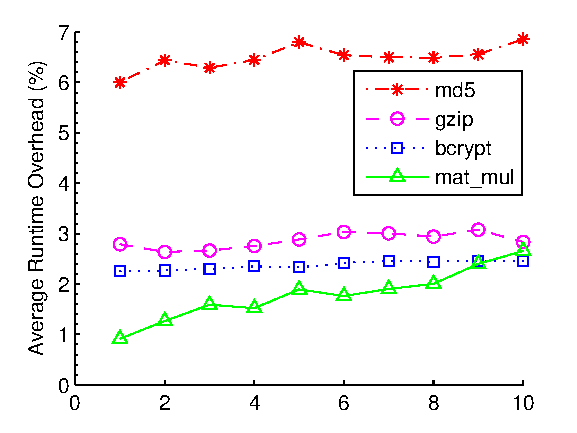
\includegraphics[width=0.9\textwidth]{fig/avg_runtime.pdf}
%\caption{The average runtime overhead per dynamically executed critical instruction.}
%\label{fig:avgruntime}
%\end{minipage}
%\end{figure}
%\hspace{0.005\textwidth}
%\begin{minipage}[t]{0.45\linewidth}
%\begin{figure}[t]
%\centering
%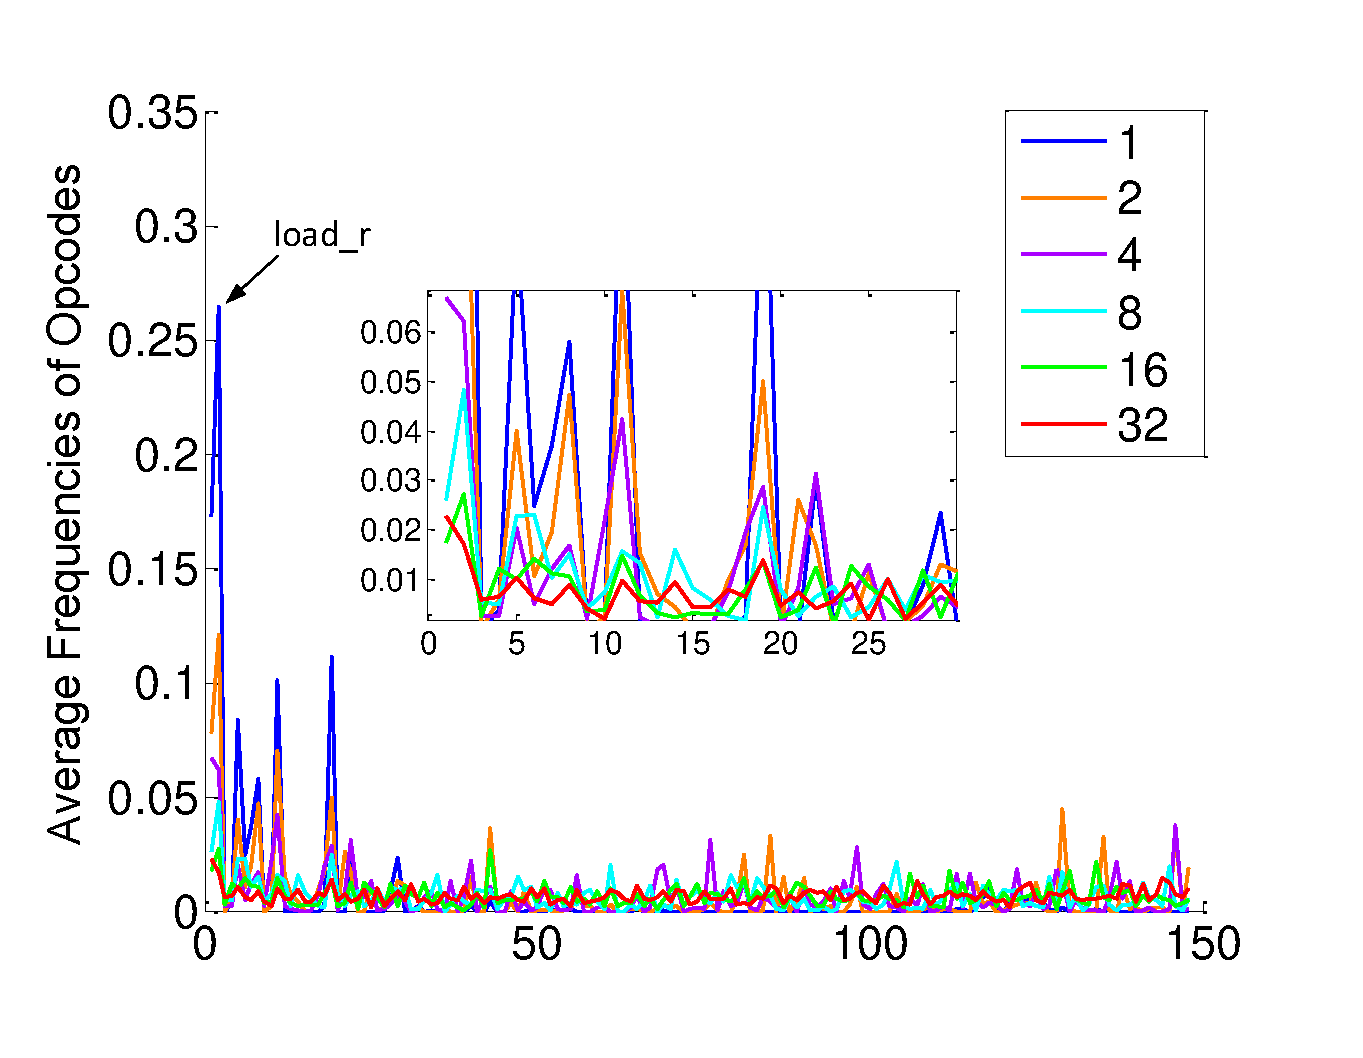
\includegraphics[width=0.9\textwidth]{fig/opfreq.pdf}
%\caption{The average frequencies of \textit{opcodes}. The horizontal axis specifies the \textit{opcodes}.}
%\label{fig:freq}
%\end{minipage}
%\end{figure}


We evaluate the average runtime overhead per dynamically executed instruction.
We use $T_{ob}$ to denote the execution time of a obfuscated program,
$T_{o}$ for that of the original program,
and $C_{e}$ for the count of the critical instructions been dynamically executed.
The average runtime overhead per dynamically executed instruction is calculated by
%\[\frac{T_{ob} - T_{o}}{C_{e}}.\]
\[(T_{ob} - T_{o})/C_{e}. \] The results are shown in figure \ref{fig:avgruntime}.
From this figure, we can learn that \texttt{md5} has the largest
average runtime overhead per dynamically executed instruction.
The reason is that the critical code of \texttt{md5} is full of arithmetical and logical instructions,
which takes a longer time to interpret.


\begin{figure}[!t]
\centering
\begin{minipage}[t]{0.45\linewidth}
\centering
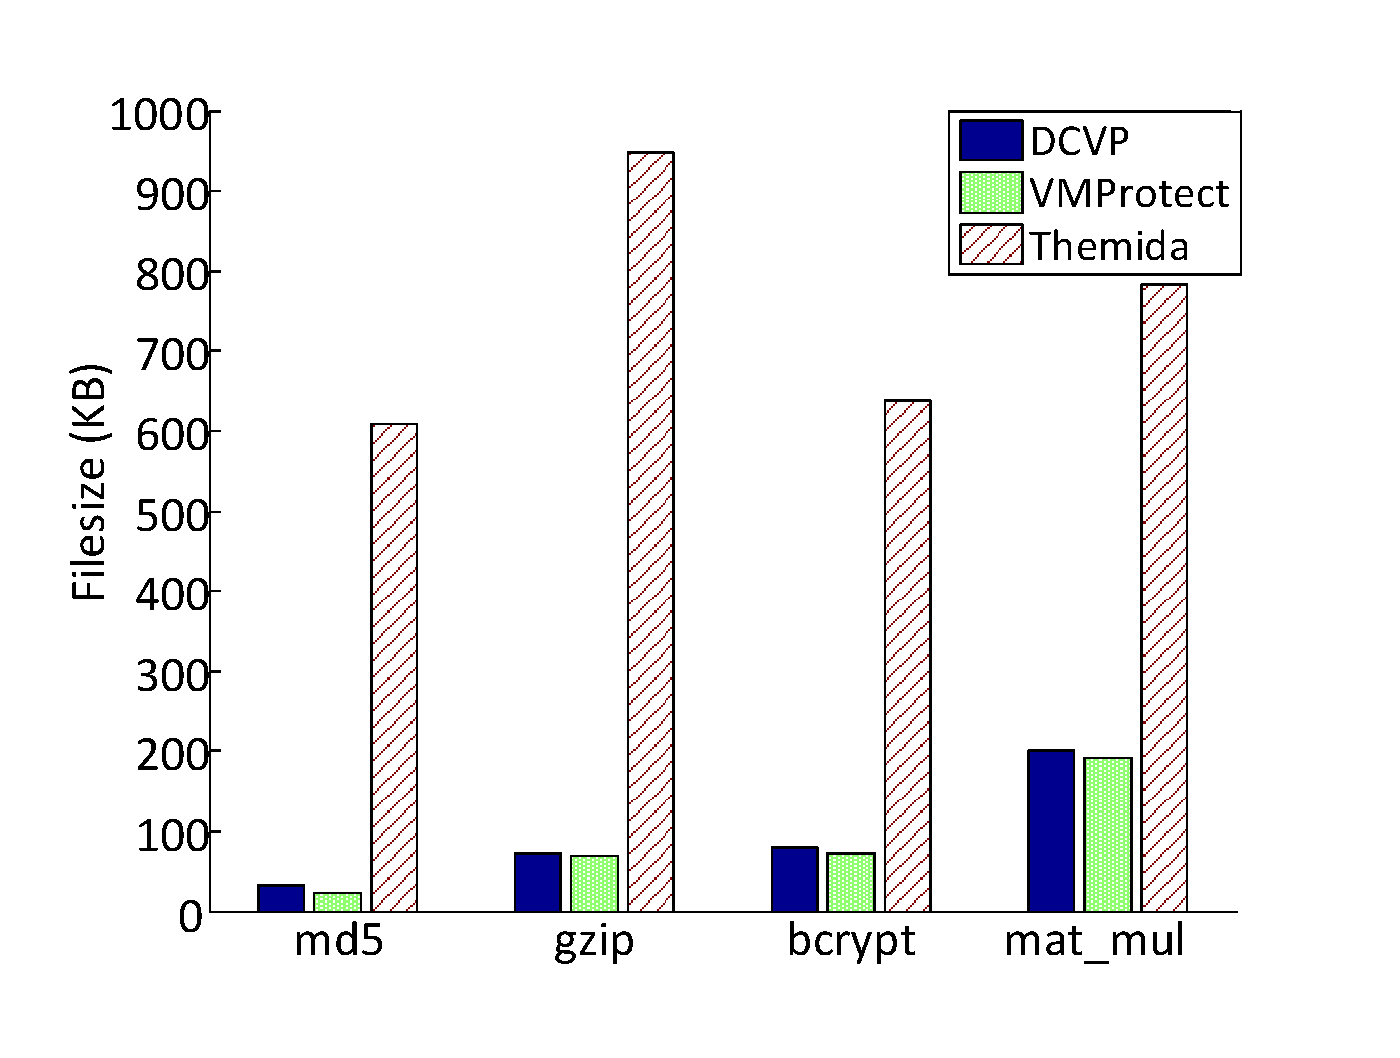
\includegraphics[width=0.9\textwidth]{fig/figfilecom.pdf}
\caption{The comparison of impact on file size (KB) with VMProtect and Themida.}
\label{fig:filecom}
\end{minipage}
%\end{figure}
\hspace{0.005\textwidth}
\begin{minipage}[t]{0.45\linewidth}
%\begin{figure}[t]
\centering
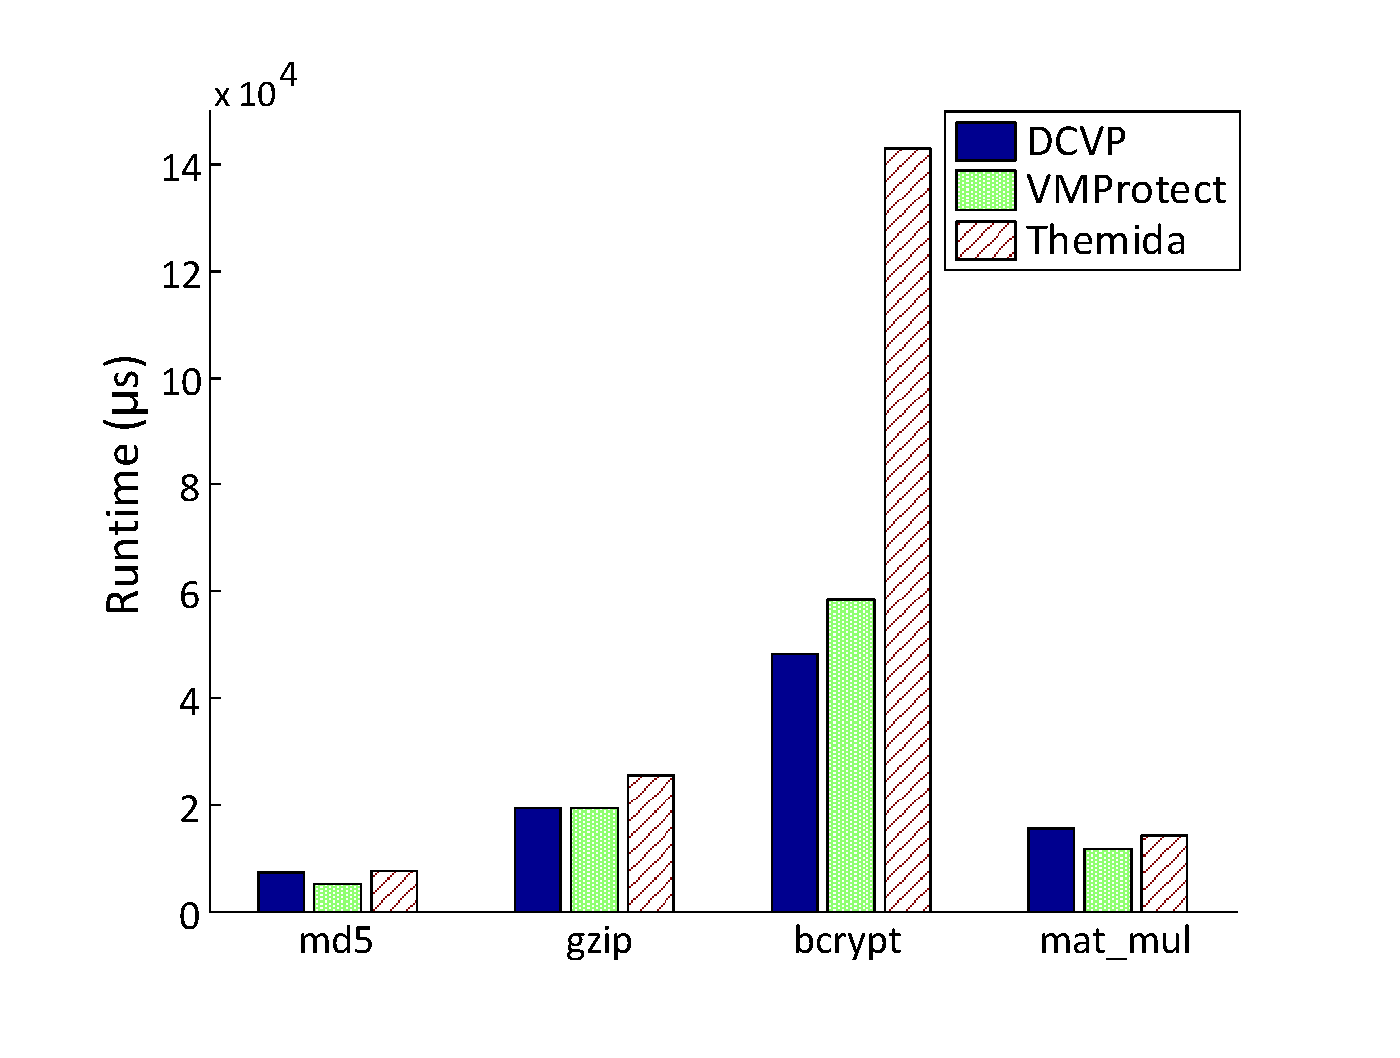
\includegraphics[width=0.9\textwidth]{fig/figtimecom.pdf}
\caption{ The comparison of runtime performance ($\mu$s) with VMProtect and Themida.}
\label{fig:timecom}
\end{minipage}
\end{figure}



Finally, we use two commercial code virtualization protection system for comparison,
VMProtect~\cite{vmp} and Themida~\cite{Themida}.
Figure~\ref{fig:filecom} shows the impact of the three virtualization protection system
on the file size of the four target programs.
The cost of Themida is much greater than the other two system,
and the impact of DCVP and VMProtect is similar.
This result should be related to the design of virtual instructions and \texttt{handlers}.
Runtime overhead as shown in Figure~\ref{fig:timecom}.
In general, the effects of the three protection systems are similar.
Special, the runtime overhead of \texttt{bcrypt} that protected by Themida
is far greater than the other target programs.
This may be related to the design of the Themida and the executed number of critical instructions in \texttt{bcrypt}.
According to above comparison, we can see that DCVP is similar to VMProtect in temporal and spatial overhead, and they are all better than Themida.


\section{Related Work}\label{sec:related}
Software protection is used to protect the intellectual property encapsulated within software programs
from been understood and modified, by transforming target program into a more obscure and hard-understanding one.
The earliest published works in software protection can be traced back to 1980,
Kent \cite{kent1981protecting} addressed the security requirements of software vendors:
protection from software copying and modification.
During the past decades, numerous approaches of software protection have been proposed,
e.g. junk instructions, equivalent instructions \cite{nicolaou2009applied}, packer (such as,
\texttt{ASProtect}~\cite{asprotect},
\texttt{UPX}~\cite{upx}),
code encryption, control flow and data flow obfuscation \cite{collberg2002watermarking,liem2008compiler,ge2005control}, etc.
These conventional approaches alone provide only limited obscurity,
and one protection system usually integrates several of these and makes them work together to provide a certain level of obscurity.

In recent years, there have been many different code protection technology.
Such as, control flow integrity~\cite{Zhang2013Practical,Zhang2013Control} provide a strong protection
against modern control flow hijacking attacks, including those based on Return-Oriented Programming (ROP).
Code Randomization, Stephen Crane et al.~\cite{Crane2015Readactor} presents a practical, fine-grained code randomization defense,
called Readactor, resilient to both static and dynamic ROP attacks.
At the same time, the code reverse analysis technology is developing.
Symbolic and concolic execution~\cite{Yadegari2015Symbolic} and Data flow tracking and tanit
analysis~\cite{Jee2012A,Balliu2014Automating,Yadegari2015A} can find important applications
in a number of security-related program analyses, including analysis of malicious code.
This paper focuses on the code virtualization protection and its reverse analysis technology.


Code virtualized obfuscation, has recently been used to protect software from malicious reverse engineering \cite{cv,vmp,fang2011multi,wang2014tdvmp,wang2013nislvmp}.
In Section~\ref{sec:background} and~\ref{sec:threat-model} we have already introduced the details of VM-based obfuscation and possible attacks.
Existing researches on VM-based obfuscation focus on foiling reverse analysis.
TDVMP \cite{wang2014tdvmp} obfuscates \texttt{handlers} to generate multiple semantics-equivalent
but appearance-different ones and embeds them into target program.
At runtime, it will execute different instructions since the execution of each \texttt{handler}
is chose from the several candidates randomly, i.e., the obfuscated program has a per-process execution diversity.
This is especially useful for defeating dynamic analysis.
Fang et al. \cite{fang2011multi} presented a multi-stage obfuscation method that iteratively transforms a program
for many times in using different interpretations.
DCVP focuses on invalidating the analysis knowledge about the semantics of bytecode instructions
and preventing from quick and large scale reverse analyses,
which is orthogonal to the above approaches and is complementary to them.


Has been also have some deobfuscation techniques of code virtualization was put forward. Representative like,
Sharif et al.~\cite{sharif2009automatic} used dynamic data-flow and taint analysis to identify data buffers
containing the bytecode program and extract the syntactic and semantic information about the bytecode instructions.
Coogan et al.~\cite{coogan2011deobfuscation} proposed an approach to identify instructions that related to system calls, and automatically extract an approximate dynamic trace of the original code.
Yadegari et al.~\cite{Yadegari2015A}, proposed an approach to track the flow of inputs values, and then use
semantics-preserving code transformations to simplify the logic of the instructions.
These approach, however, or can only extract some execution characteristics of target program
and can not restore the structure of the original code completely,
or needed taint analysis to track and analyze the data flow,
and this process may be impeded by enforcing dataflow obfuscation to the handling procedures~\cite{liem2008compiler}.
These methods are limited more or less.

DCVP adopts ISR (Instruction Set Randomization) techniques while generating randomized and distinct virtual instruction sets.
ISR has been used to prevent code injection attacks by randomizing the underlying system instructions~\cite{barrantes2003randomized,kc2003countering,portokalidis2010fast}.
In this approach, instructions are encrypted with a set of random keys and
then decrypted before being fetched and executed by the CPU.
ISR is effective for defeating code injection attacks but cannot prevent from reverse engineering attacks.
As in our attack model, software programs are executed in a malicious host environment,
where attackers are able to trace and log the decrypted instructions for later analysis.
DCVP employs an approach similar to ISR while generating random virtual instruction sets,
by changing the relationship between the opcodes and the virtual instructions~\cite{kc2003countering},
but it never ``decrypts" the virtual instructions back into their original ones.
Instead, DCVP uses \texttt{handlers} to interpret the virtual instructions.
and the \texttt{handlers} of virtual instructions are more complex than their corresponding native instructions.
Besides, DCVP uses the multiple partitions and has the different ISRs in a single program,
making the reverse analyses even more difficult and tedious.



\section{Conclusion}
In this paper, we have presented the DCVP, a VM-based code obfuscation scheme.
DCVP is designed to prevent code reverse engineering attacks
that use knowledge obtained from programs protected under the same code obfuscation technique.
We achieve this by first partitioning the protected code region to different segments;
then randomly mapping the opcode of each virtual instruction from different segments to different bytecode handlers.
As a result, the mapping between a virtual instruction and native code changes from one code segment to the other.
This significantly increases the diversity of the program behavior,
making it much harder for an attacker to reuse knowledge obtained from other programs to attack the target application.
We have evaluated our approach on a set of real-world applications
and compared it against state-of-the-art VM-based code protection tools.
Experimental results show that DCVP provides stronger protection (measured by the how likely a virtual instruction within two segments is mapped to the same native code or handler) at the cost of little extract overhead.
% Start of "Sample References" section



% Appendix

% Acknowledgments
\begin{acks}
This work was partial supported by projects of the National Natural Science Foundation of China (No. 61373177, No. 61572402),
the Key Project of Chinese Ministry of Education (No. 211181),
the International Cooperation Foundation of Shaanxi Province, China (No. 2013KW01-02, No. 2015KW-003, No. 2016KW-034),
the China Postdoctoral Science Foundation (grant No. 2012M521797),
the Research Project of Shaanxi Province Department of Education (No. 15JK1734),
the Research Project of NWU, China (No. 14NW28),
and the UK Engineering and Physical Sciences Research Council under grants EP/M01567X/1 (SANDeRs), EP/M015793/1 (DIVIDEND).
\end{acks}

% Bibliography
\bibliographystyle{ACM-Reference-Format-Journals}
\bibliography{DCVP_bib}
                             % Sample .bib file with references that match those in
                             % the 'Specifications Document (V1.5)' as well containing
                             % 'legacy' bibs and bibs with 'alternate codings'.
                             % Gerry Murray - March 2012

% History dates
%\received{October 2016}{March 2017}{June 2017}

\end{document}


